\subsection{Shear reinforcement}
Provisions for shear reinforcement at slab-column connections for non-SFRS members were adapted in \cite{aci31805} to reduce slab punching shear failure likelihood. \citet[Section 18.14.5]{aci31819} states for nonprestressed slabs that design story drift ratio is limited to the following
\begin{equation}\label{eqdr}
\frac{\Delta_x}{\mathbf{h_{sx}}}\ge\mathbf{0.035-0.05\frac{v_{uv}}{\phi v_c}}
\end{equation}
presented in \ref{fr181451}.
If the drift ratio exceeds this amount(\ref{eqdr}) thus slab shear reinforcements either stirrups or headed studs should be provided at any slab critical section considering that $\mathbf{v_{uv}}$ is evaluated with load combinations including earthquake effect $\mathbf{E}$ and $\Delta_x/\mathbf{h_{sx}}$\footnote{$\mathbf{v_{uv}/(\phi v_c)}$ is otherwise known as the ratio between the acting vertical shear force and the punching shear resistance or Gravity shear ratio (GSR) in the literature. Larger GSRs imply lower frame or structure horizontal deformation or drift capacity and are possible with shear reinforcement\citep{gouveia2019}.} is the greater of values for adjacent stories above and below the slab-column connection while $\mathbf{v_c}$ is evaluated as below. 
\begin{equation}\label{eqt22652}
\mathbf{v_c} = \min{\left[\begin{array}{c}
1\\
1/2+{1}/{\beta}\\
1/2+{\alpha_sd}/{4b_o}\\
\end{array}\right]}
\frac{\lambda_s\lambda\sqrt{f'_c}}{3}
\end{equation}
where $\beta$ is the ratio of long to short column sides or supporting element, $\mathbf{\alpha_s}$ is the factor accounting for connection location, $\mathbf{d}$ is the slab effective depth, $\mathbf{\lambda_s}$ is the size effect factor, and regardless of shear reinforcement the critical section perimeter $\mathbf{b_o}$ is at least $\mathbf{d/2}$ away from column edges or changes in slab thickness minimizing $\mathbf{b_o}$ while with shear reinforcement an extra critical section $\mathbf{d/2}$ away from the outermost peripheral line of shear reinforcement considering the shape should be a polygon minimizing $\mathbf{b_o}$ is added\footnote{There will be two critical sections for shear reinforced sections.}, 
\begin{equation}\nonumber\begin{array}{rl}
\lambda_s =& \sqrt{{2}/({1+0.004d})}\ge1, \lambda = 1\\
\alpha_s =&\left\{\begin{array}{ll}40&\mathrm{interior}\\ 30& \mathrm{edge}\\20&\mathrm{corner}\end{array}\right.\,\mathrm{columns}
\end{array}
\end{equation}
Development of \ref{eqt22652} is reviewed in \cite{bayrak2009two}. Also note that most of the existing research on punching shear are based on test results from reinforced concrete column and slab specimens.



\cite{megally2002,moehle1996,kang2006,kang2007} identified the likelihood of punching shear failure about the slab critical section without moment transfer considering story drift ratio and shear stress $\mathbf{v_{uv}}$ due to gravity loads and the vertical component of earthquake loads therefore no induced moment calculations would be necessary. \cite{megally2000,kang2009nonlinear,moreno2008punching,song2012effective,kruger1998punching,krueger1999influence} found that moment presence significantly decreased slab punching shear resistance  that is in line with earlier findings \citep{hawkins1974,islam1976}. The above mentioned requirement (\ref{fr181451}) can also be satisfied by increasing slab thickness, changing the design to reduce story drift ratio, or a combination of all of the above. 
    
The shear reinforcement in the slab critical section should provide $\mathbf{v_s\ge0.29\sqrt{f'_c}}$ extending at least four times the slab thickness from the support face adjacent to it. In case the above requirements are not met for two-way slabs that are designated as part of SFRS \citet[Section 18.4.5.8]{aci31819} states that two-way shear stress caused by factored gravity loads without moment transfer should not exceed $\mathbf{0.4\phi v_c}$ beyond which nonprestressed slab-column connections in laboratory tests by \cite{pan1989} exhibited reduced lateral displacement ductility. 
\begin{figure}\centering
    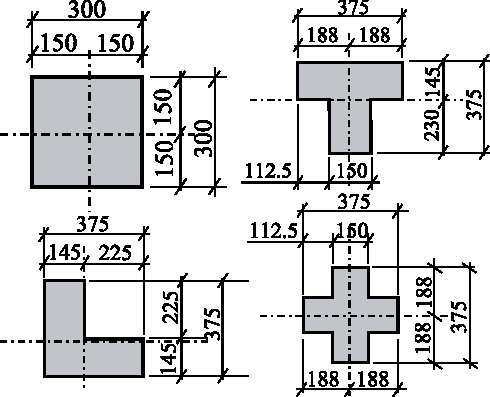
\includegraphics[width=\columnwidth]{Figures/akt1.pdf}\caption{Model column geometries\citep{akinpelu2023}.}\label{akt1}
    \end{figure}

Variety in shear reinforcement lies partly on a practical point, when various construction limitations arise such as difficulties in proper bar placement or improper stirrup configurations after slab reinforcement is done or even shear head sections barring essential reinforcement in the column and slab considering the \cite{ACI31814} requirements such as uninterrupted inserts. 

\cite{moe1961} tried to increase column effective size placing steel plates with a certain overhang as illustrated in \ref{h74f1}(a) over the column and was successful at achieving increased capacity noting that shear was concentrated on plate corners. \cite{hawkins1968} studied the bearing strength of these steel plates and proposed a plate thickness formula to provide maximum increase in column effective size without disadvantageous corner effects. 

\cite{akinpelu2023} carried out a numerical study of column shape effect on flat slab punching shear behavior implementing the finite element package ABAQUS\citep{abaqus} in which the authors tried `L', `T' and `+' shaped column geometries maintaining the column area and perimeter also introducing damage plasticity into the model(\ref{akt1}). The simulation results of \cite{akinpelu2023} showed that  the `+' geometry renders a larger column effective size and thus behaves better than others in comparison to rectangular sections\citep{akinpelu2023}. 
\cite{xue2022} investigated the punching shear behavior of reinforced concrete slab-column connections with `L' shaped columns through an experimental study with four tests followed by a numerical simulation and analysis using the finite element package ABAQUS(\ref{x2022f2}).
    \begin{figure}\centering
        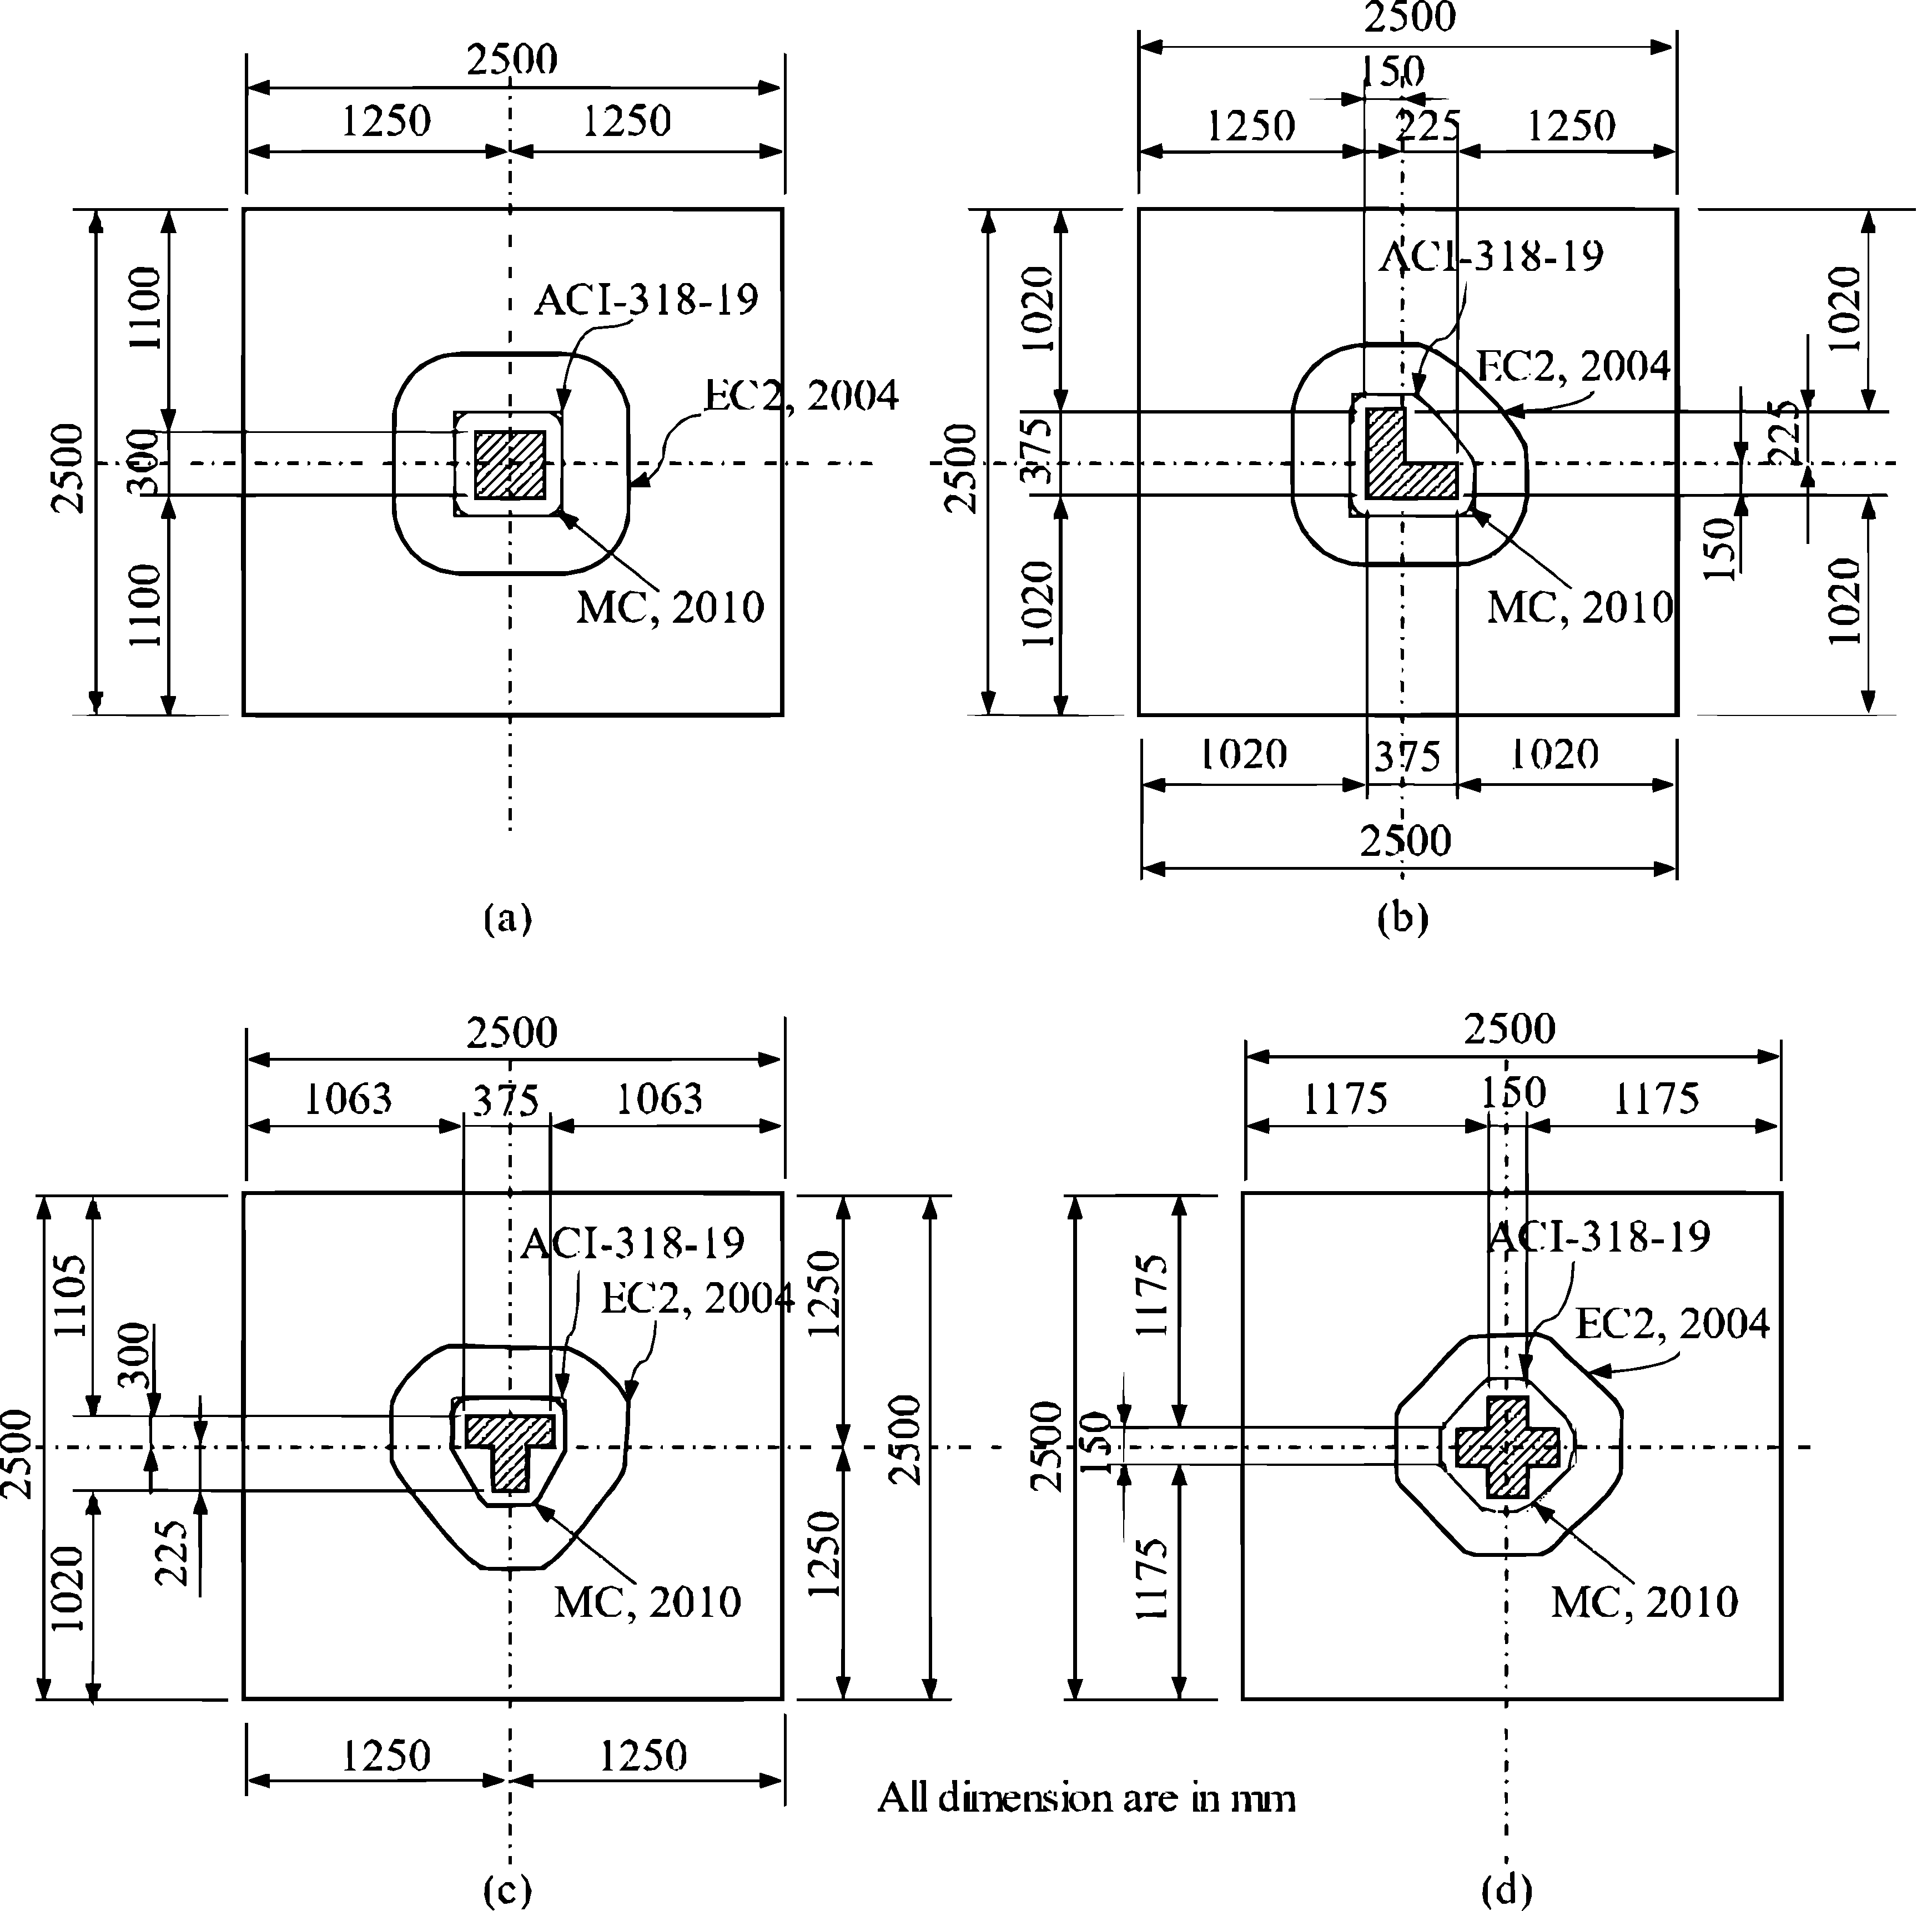
\includegraphics[width=\columnwidth]{Figures/akf3.pdf}\caption{Layouts of modelled flat slabs showing critical sections as per various code provisions, adopted from \citep{akinpelu2023}; a) Square column; b) $\mathrm{L}$; c) $\mathrm{T}$; d) $\mathrm{+}$.}\label{akf3}
        \end{figure}
    \begin{figure*}\centering
        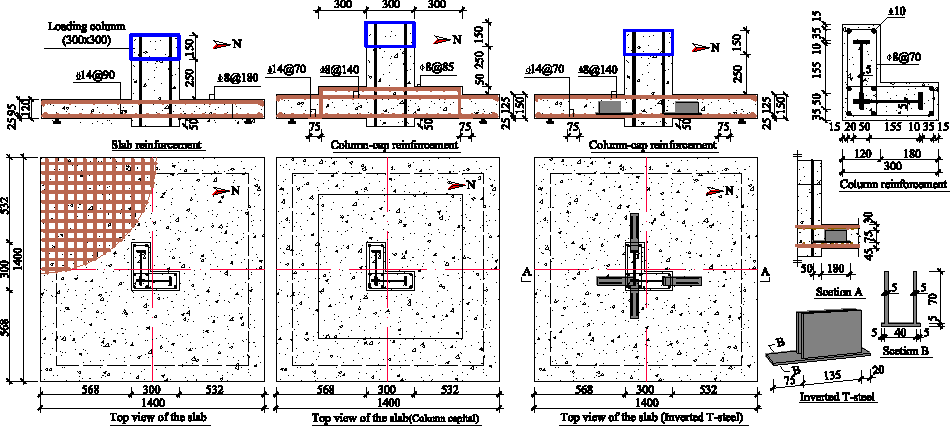
\includegraphics[width=\textwidth]{Figures/x2022f2.pdf}\caption{Specimen reinfocement detail and layout\citep{xue2022}.}\label{x2022f2}
        \end{figure*}
\subsubsection{Shearheads}
\begin{figure}\centering
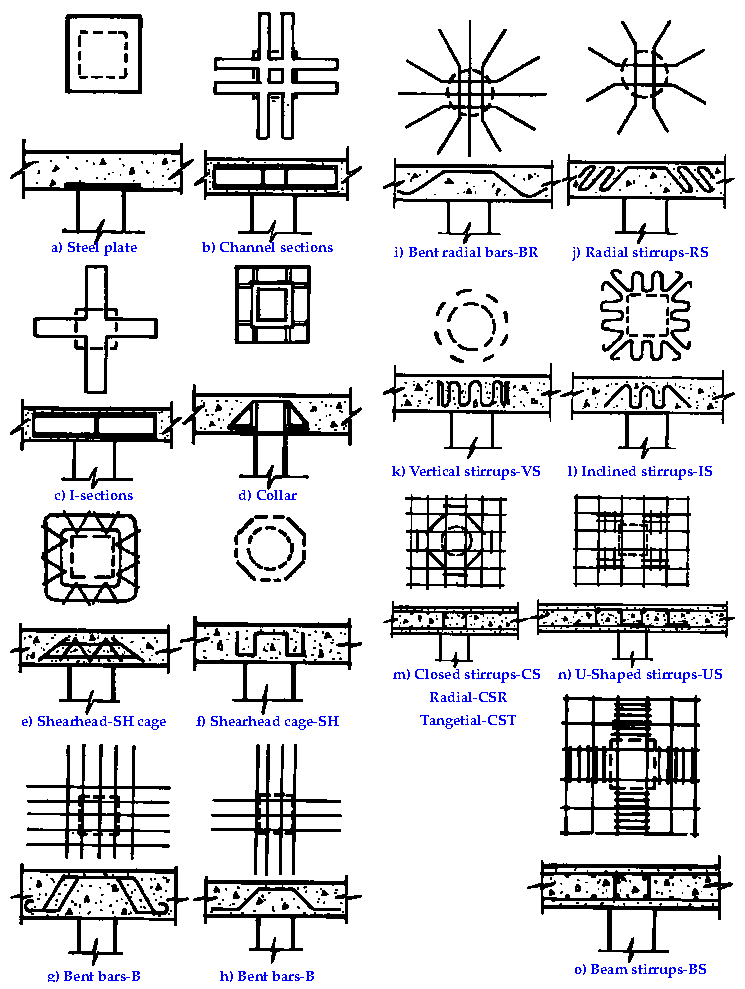
\includegraphics[width=\columnwidth]{Figures/tikzout/h74f1m.pdf}
\caption{Shear reinforcements\citep{hawkins1974a}; a) Steel plate\citep{moe1961}; b) Channel sections\citep{hawkins1974}; c) $\mathrm{I}$ sections\citep{hawkins1974}; d) Collar\citep{tasker1963}; e) Shearhead-SH, cage; f) Shearhead cage-SH; g,h) Bent bars-B; i) Bent radial bars-BR; j) Radial stirrups-RS; k) Vertical stirrups-VS; l) Inclined stirrups-IS; m) Close stirrups-CS, Radial-CSR, Tangential-CST; n) U-shaped stirrups-US; o) Beam stirrups-BS.}\label{h74f1}
\end{figure}

Shearheads are another type of shear reinforcement that despite being originally introduced in \cite{wheeler1936} are seldom used in current practice so their design provisions have been omitted in \cite{aci31819} and may be designed following \cite{ACI31814} provisions. Design criteria in \cite{aci31871} were developed based on shear forces in \cite{hawkins1974,corley1968} who performed 21 tests, 16 of which were with cruciform grillages of $\mathrm{I}$ and $\mathrm{C}$ steel sections complementing \cite{corley1968,hawkins1974}(\ref{h74f1} b,c) and the approach has been maintained up to \cite{ACI31814}. Results from \cite{hawkins1974a} contrasted with \cite{aci31871} provisions and \cite{hawkins1974} also showed that after cracking in the slab around the connection the subsequent shear forces applied are carried by the shearhead module while failure initiates either through punching along the shearhead perimeter or reaching the shearhead flexural capacity. Commentary on \citet[Section 22.6.9]{ACI31814} suggests that a minimum flexural strength should be provided to ensure slab shear strength is reached before shearhead flexural strength is exceeded. The above mentioned shearheads (\ref{h74f1} b,c) increased slab shear capacity as shearhead arm length grew thus \cite{corley1968,hawkins1974} introduced the critical sections and equations for column face moment and shear illustrated in \ref{fr2269814}. These results were adopted by \cite{Al-hamd2018} who proposed two new shearhead designs (\ref{ahf5}) based on nine laboratory tests with eccentrically loaded specimens with an offset corbel (\ref{ahf4}) similar to \cite{kruger1998} followed by a numerical study of connection behavior. Load and moment in the manner described by \cite{kruger1998,Al-hamd2018} is quite advantageous compared to \cite{ghali2000stud,kang2009nonlinear,moreno2008punching,song2012effective,hawkins1974,islam1976} who produced moments by applying a lateral load to one of the column sides. While reporting results from testing shearhead systems to improve steel column-flat slab connection ductility under cyclic loads \cite{EDER2012239} made a similar argument to the above pointing out that slab behavior is controlled by shearhead stiffness and high connection strength and ductility are realizable when using partially integrated shearheads if dissipative elements are designed to yield in shear first. 
\begin{figure}\centering
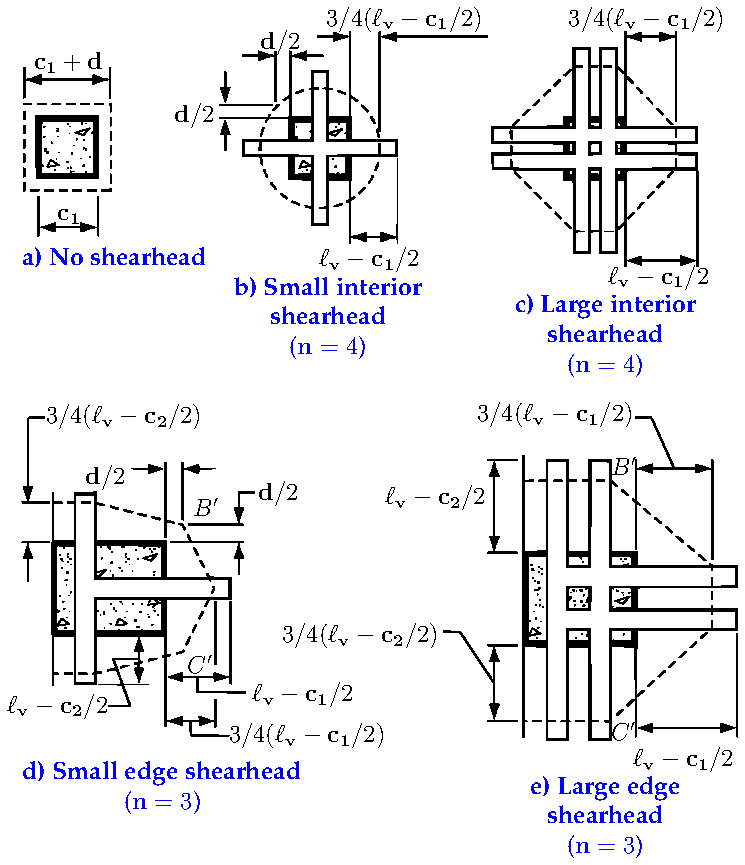
\includegraphics[width=\columnwidth]{Figures/tikzout/fr2269814.pdf}
\caption{Flat slab shear critical sections with and without shearhead adapted from \cite{ACI31814}; a,b,c) Interior columns same as \cite{hawkins1974a}; d,e) Edge columns.}\label{fr2269814}
\end{figure}
Steel columns and flat slabs are generally connected with steel inserts welded to the column and then integrated into the slab\footnote{More on this in \ref{cft}.}.

Shearhead response in accord with \ref{fr2269814} is ensured by anchoring the shearhead steel section flanges within the slab compression zone based of which \cite{aci31871} requires having the compressions flange within $0.3\mathbf{d}$ of the slab compression surface. \cite{godycki1984} showed embedment length on ultimate connection capacity for flat slabs with cruciform or $+$ shearheads under eccentric loading.

\begin{figure}\centering
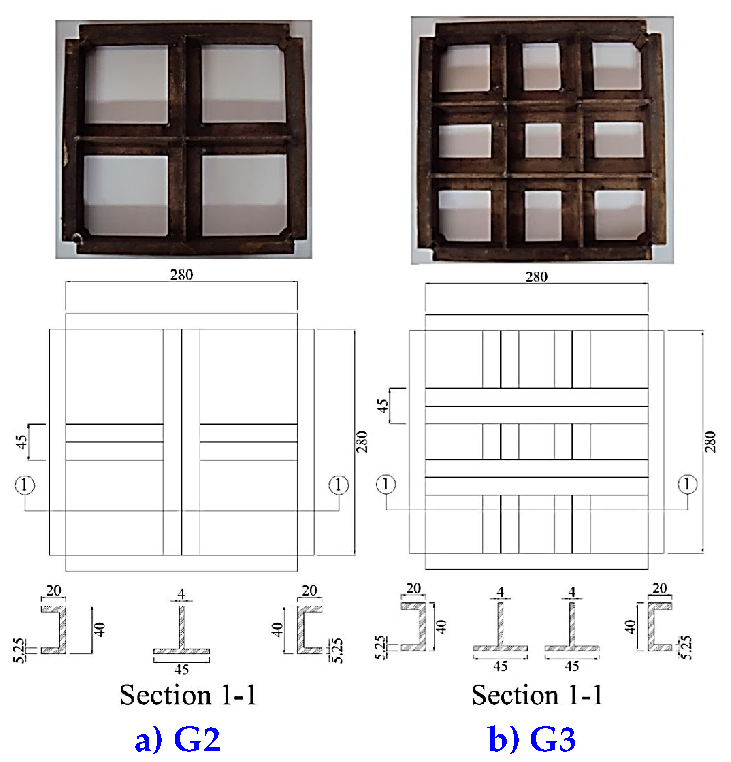
\includegraphics[width=\columnwidth]{Figures/tikzout/ahf5.pdf}
\caption{Proposed shearhead layouts by \cite{Al-hamd2018}; a) G2; b) G3. }\label{ahf5}
\end{figure}
\begin{figure}\centering
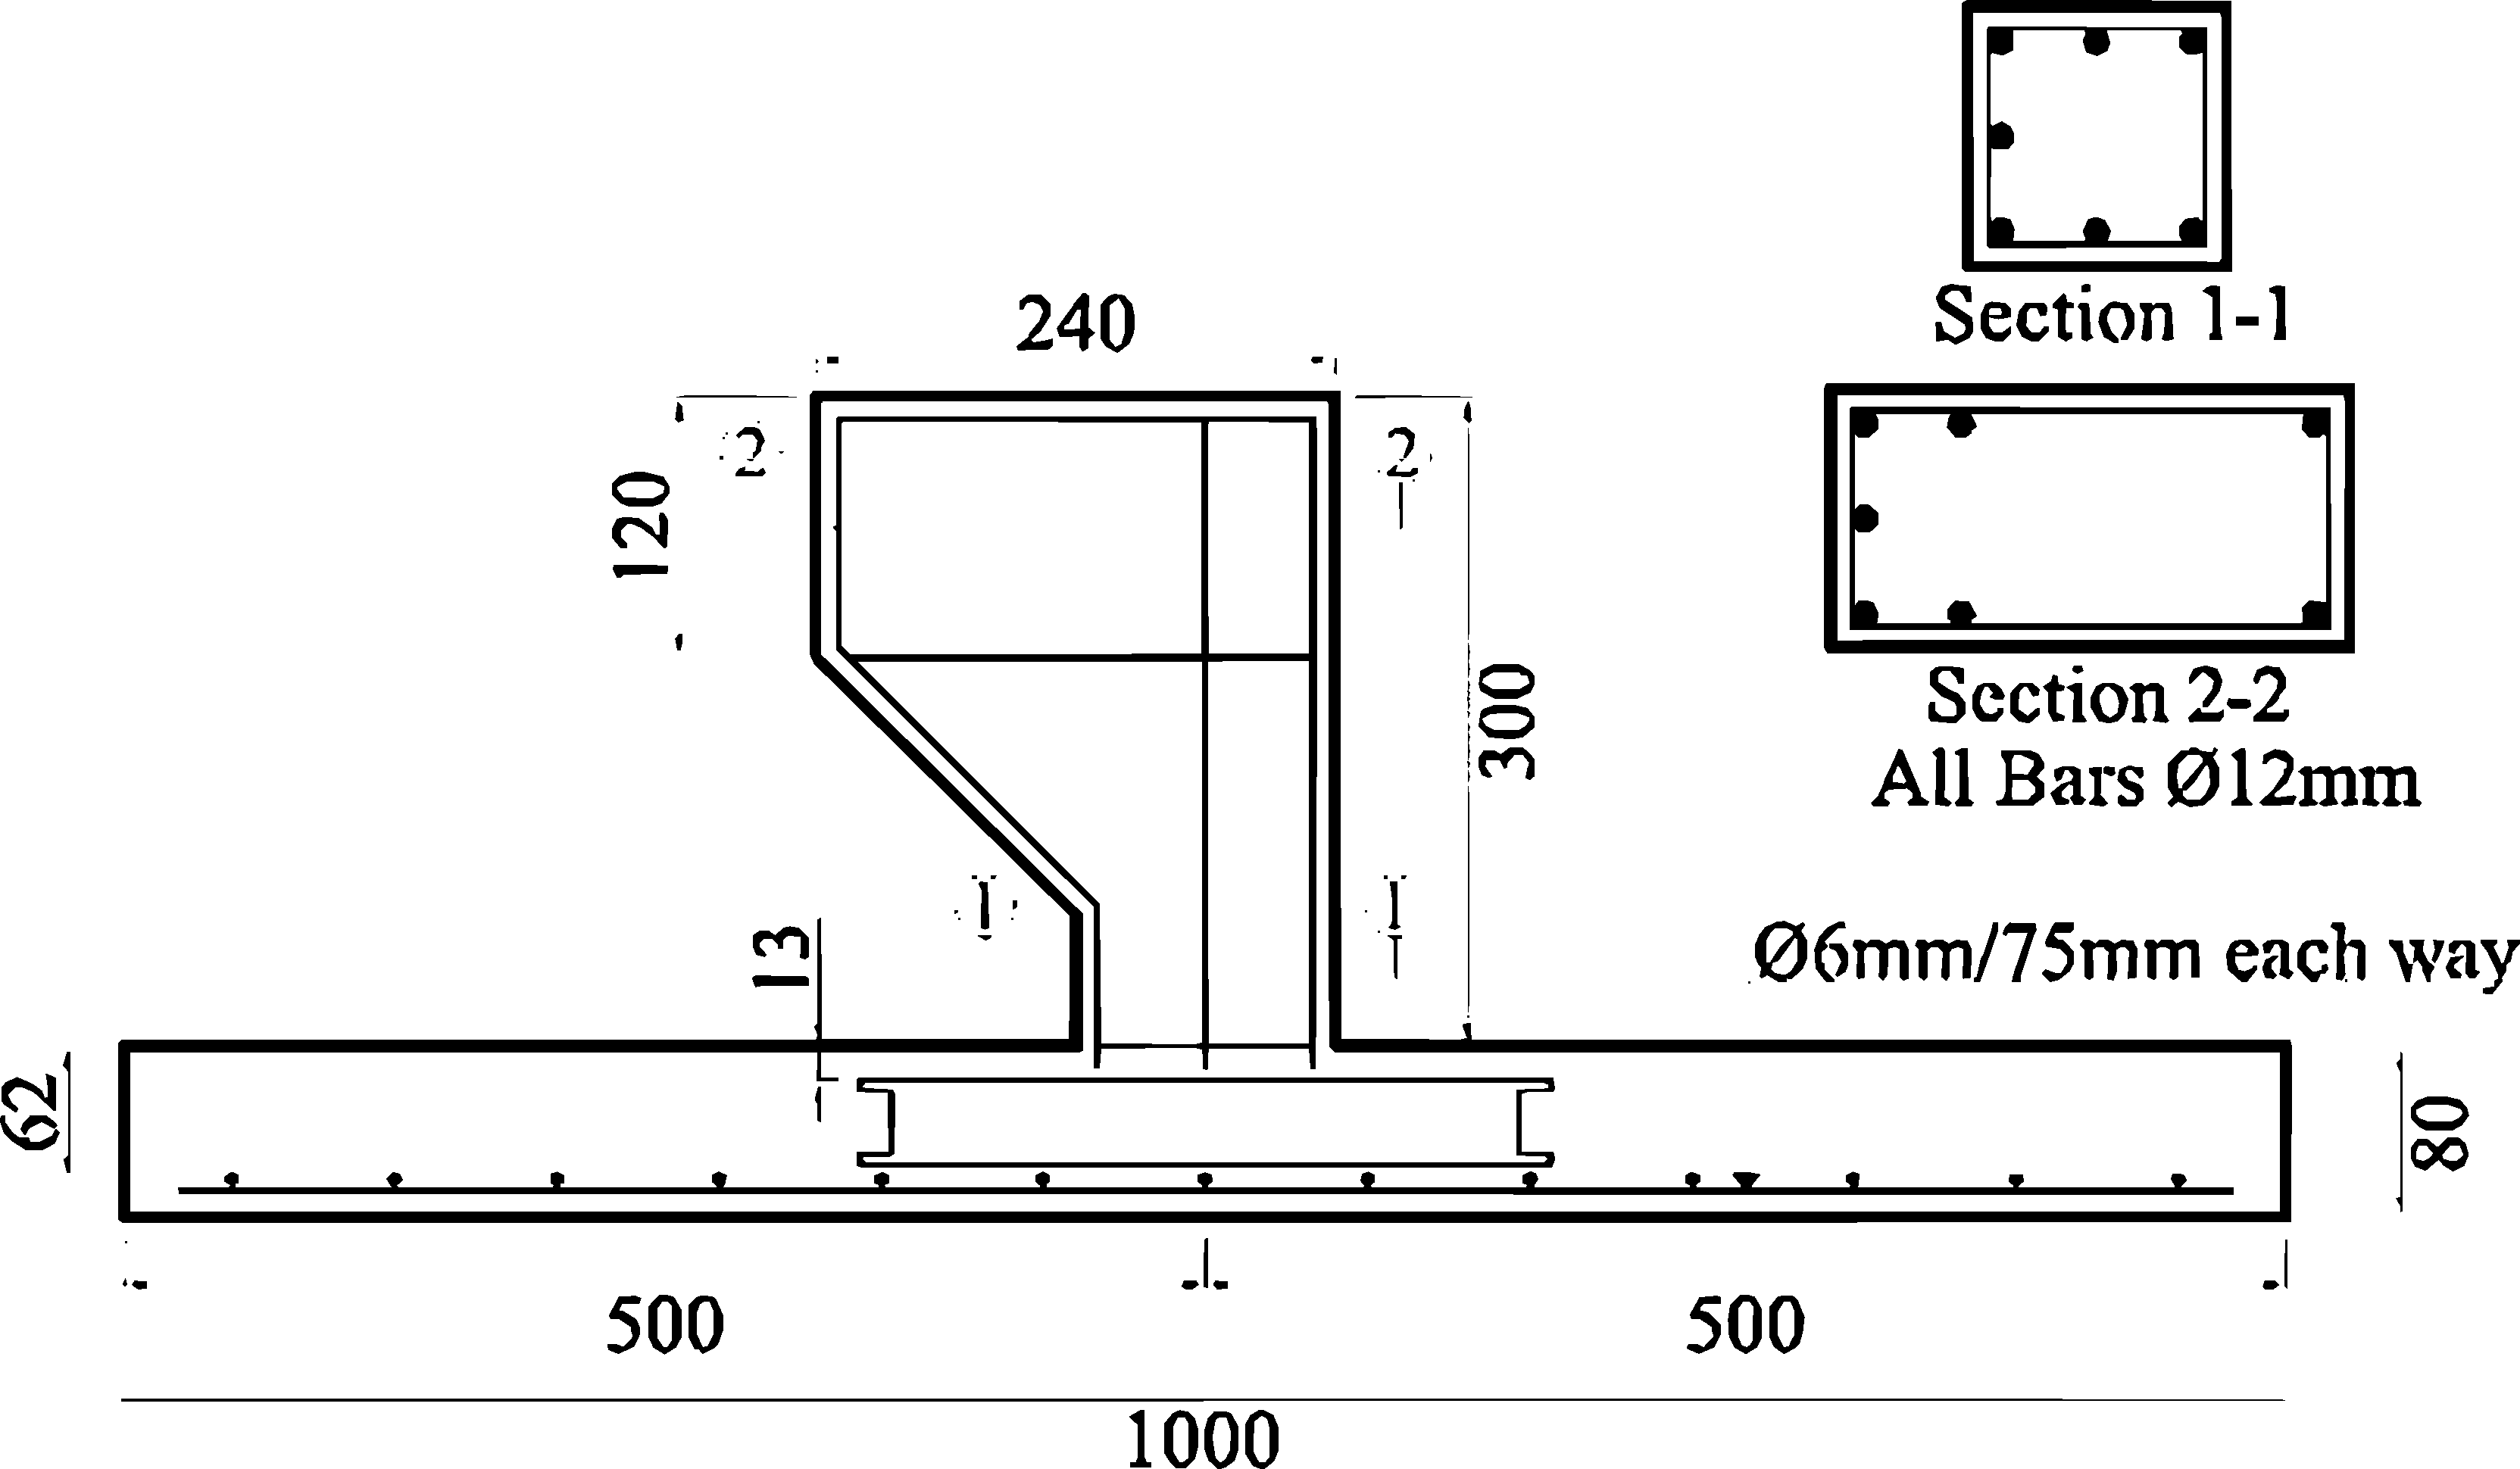
\includegraphics[width=\columnwidth]{Figures/ahf4.pdf}
\caption{Tested slab geometry with offset corbel by \cite{Al-hamd2018} (all dimensions in mm).}\label{ahf4}
\end{figure}

\cite{bompa2015} proposed a method for punching shear evaluation of reinforced concrete flat slab-column connections without shear reinforcement. Having studied shear behavior of beam to steel column assemblages\citep{bompa2016b} with a series of 5 large scale tests with shearheads or arms welded to the steel column and embeded in reinforced concrete beams, \cite{Bompa2016a} carried out six large scale tests and developed an analytical model for steel column-flat slab connection with shearheads(\ref{bf2}) that showcased the positive influence of continuity plates connecting the shearheads. The shearheads were welded to the steel column and fully embedded in the slab while in the 6 test specimens the embedment length, slab thickness and shearhead cross section were maintained whereas shearhead assemblage configuration, flexural reinforcement ratio and transverse reinforcement contributions varied. \cite{bompa2020} Carried out a a thorough three-dimensional nonlinear numerical and parametric analysis implementing the concrete damage plasticity models validated against experimental results from three test series\citep{guandalini2009punching,chana1996,hawkins1974} and proposed analytical models for connection rotational response as well as the ultimate strength of reinforced concrete slab systems provided with fully embedded shearheads(\ref{b2020f2}). 
\begin{figure}\centering
    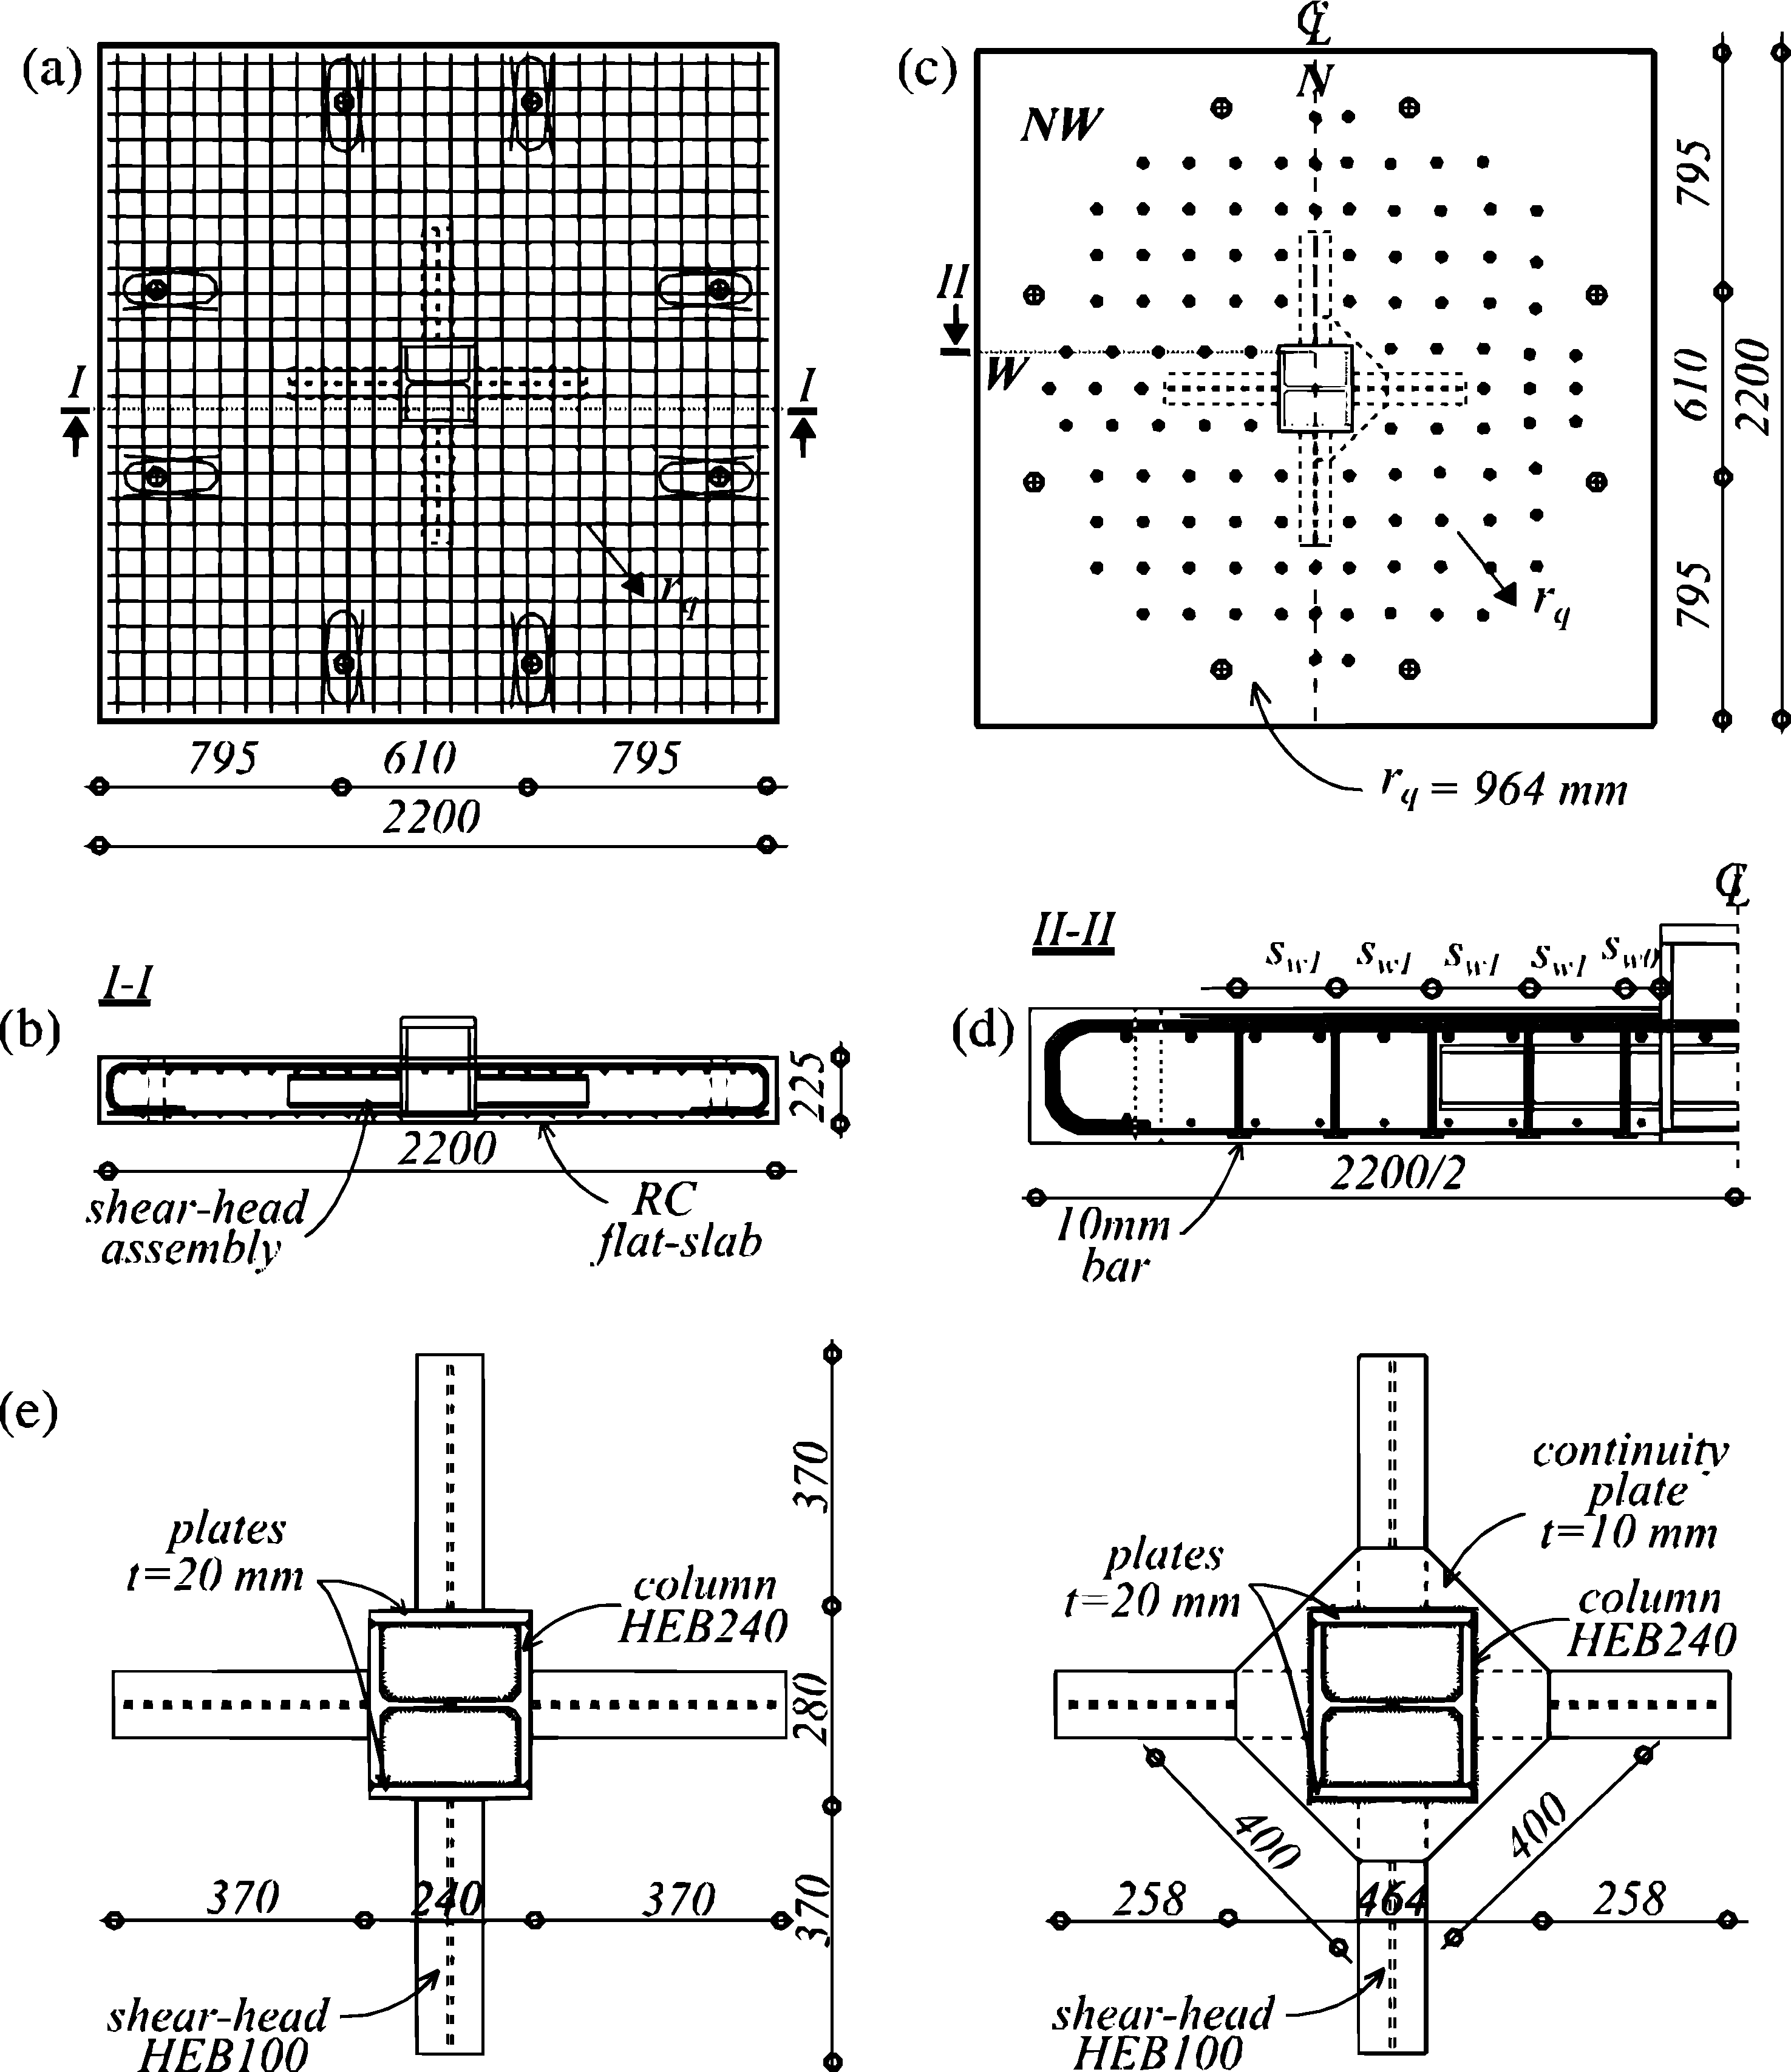
\includegraphics[width=\columnwidth]{Figures/bf2.pdf}
    \caption{Specimen arrangement \cite{Bompa2016a}; a) Longitudinal reinforcement layout; b) I-I cross-sectional view; c) transverse reinforcement layout; d) II-II cross-sectional view from transverse reinforcement; e) Shearhead details, without continuity plate on the left and with continuity plate on the right.}
    \label{bf2}
    \end{figure}
\begin{figure}\centering
    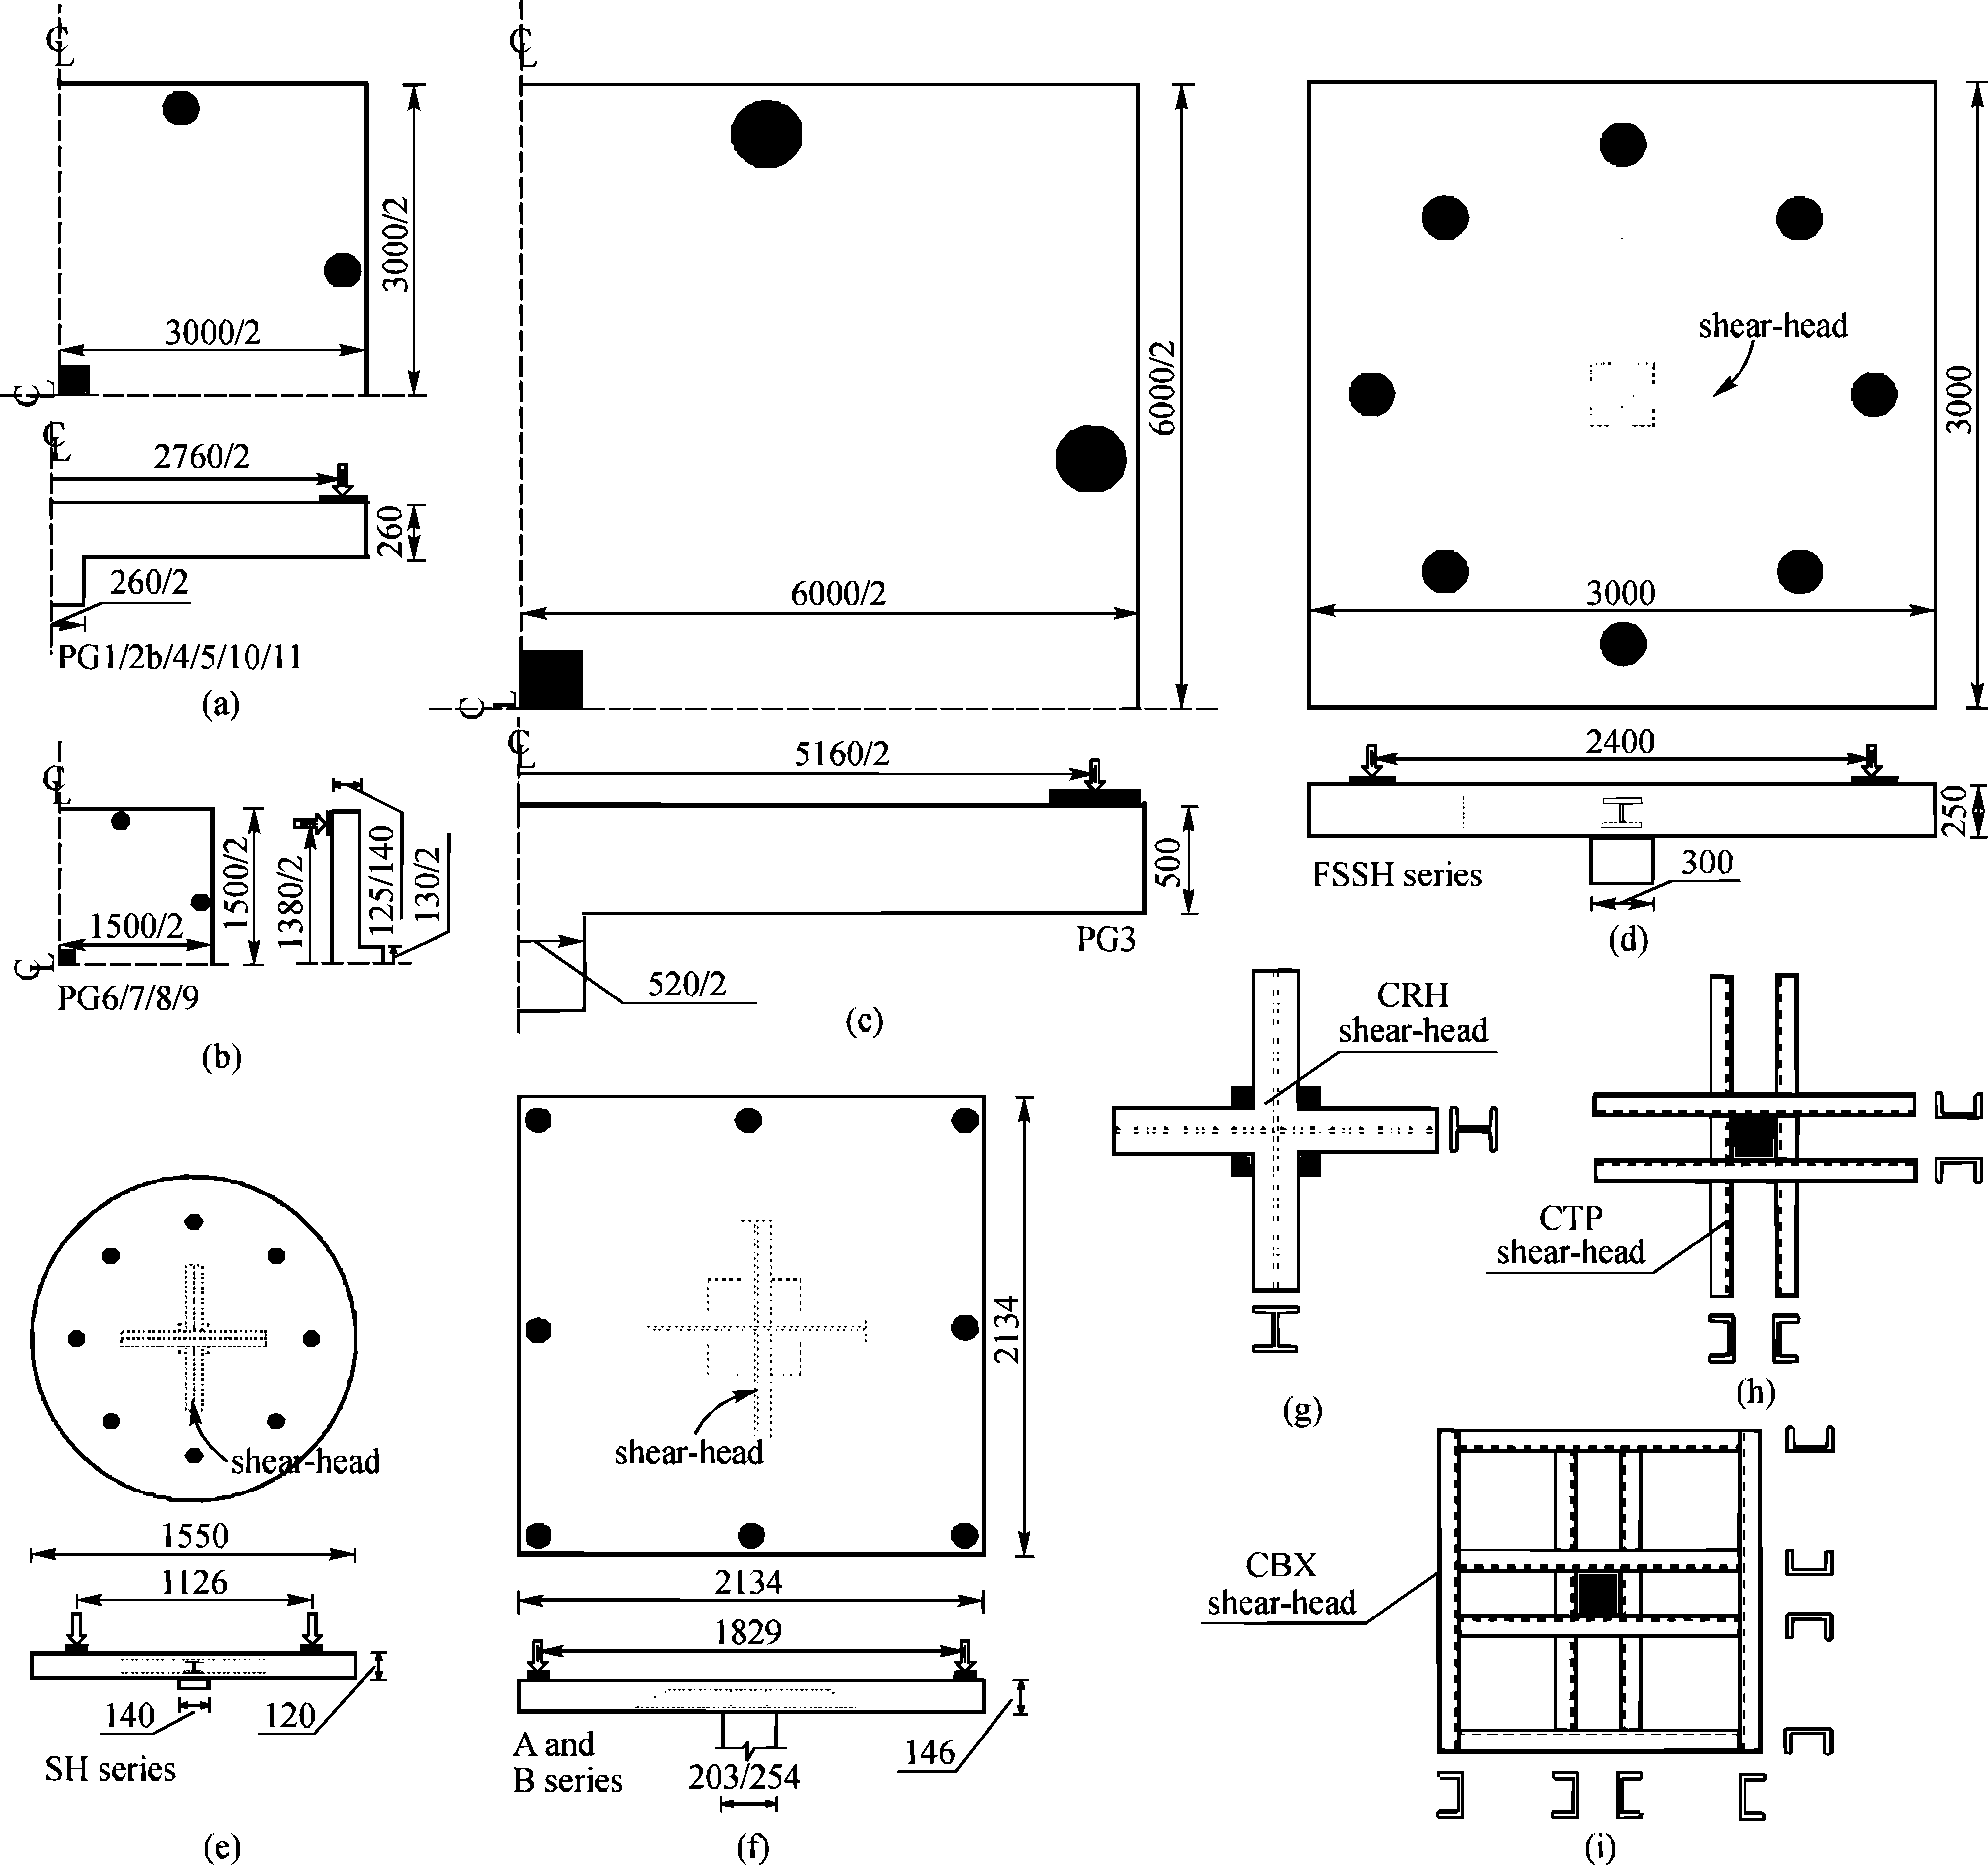
\includegraphics[width=\columnwidth]{Figures/b2020f2.pdf}
    \caption{Schematic representation of specimens numerically studied in \cite{bompa2020}; a) Full scale specimens PG1, PG2b, PG5, PG10, PG11; b) Half scale specimens PG6, PG7, PG8, PG9; c) Double scale specimen PG3 from \cite{guandalini2009punching}; d) FSSH series; e) SH series from \cite{chana1996}; f) A and B series \citep{hawkins1974}; Cruciform shear-heads made of g) Welded back-to-back channel or I sections (CRH); h) Two pairs of channels at the support region (CTP) shearheads; i) Closed-box shearheads (CBX).}
    \label{b2020f2}
    \end{figure}
\cite{eder2010} validated a nonlinear finite element model against a large-scale reinforced concrete flat slab without shear reinforcement that failed in punching and subsequently carried out a parametric analysis of key parameters. These authors modelled a large scale hybrid reinforced concrete flat slab specimen tested at the London Imperial College with a steel column and \cite{aci31808} type steel shearhead as well. Their analysis suggests that loads are principally transferred into the shearhead arm tips if the failure surface lies outside shearhead arm length while a more uniform load transfer into these arms would occur if the failure surface lies inside. \cite{EDER20111164} presented a novel partially integrated shearhead detail(\ref{e2011f3}) with a gap around the tubular steel column(\ref{e2011f4}) to enable shearhead yield in the shearhead prior to slab punching shear and compared it with the typical \cite{aci31808} shearhead presenting test results from four large-scale specimens and numerical analysis under gravity and cyclic lateral loadings following which \cite{EDER2012239} further studied the inelastic performance and design of this novel ductile steel shearhead with additional u-bars under these loads. \cite{EDER2012239} notes that I section shear arms perform better than closed box sections due to improved composite action with the slab and also suggests anchoring of the shear arms to the slab through end plates or otherwise to further resist the siginificant axial forces which arise as a result of geometric nonlinearity. 
    \begin{figure}\centering
    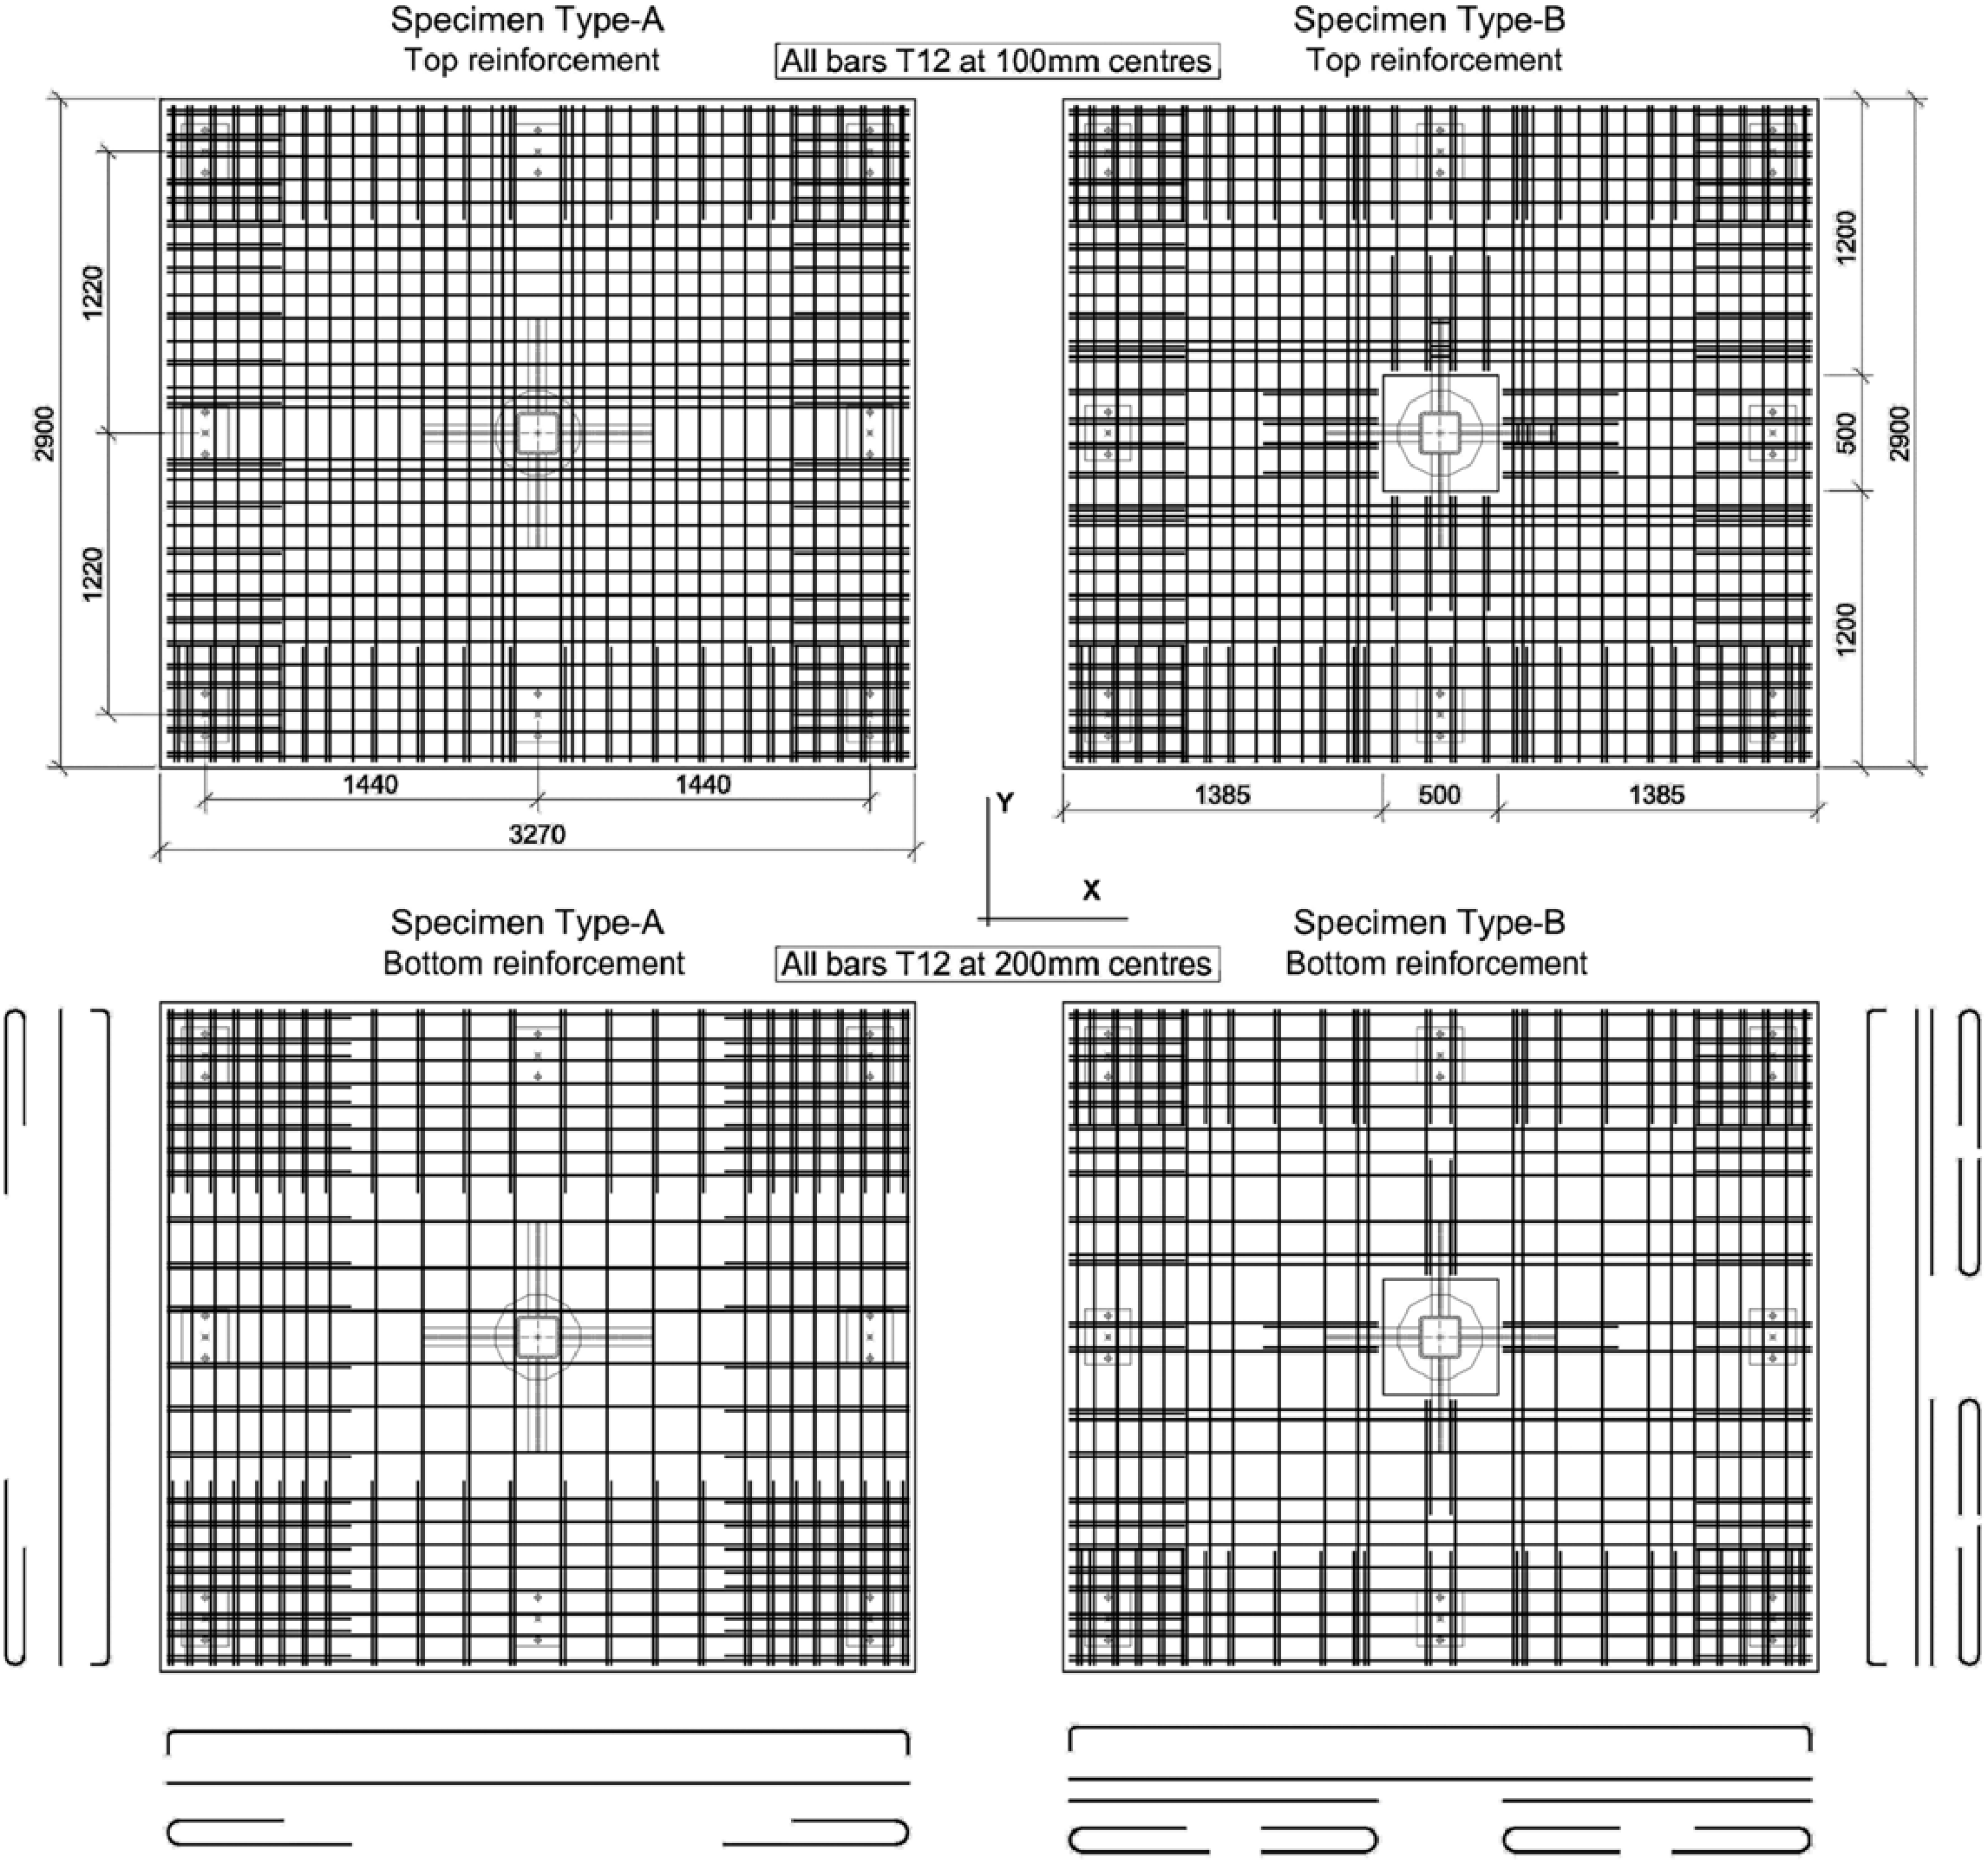
\includegraphics[width=\columnwidth]{Figures/e2011f3.pdf}
    \caption{Specimen reinforcement layouts in \cite{EDER20111164}.}
    \label{e2011f3}
    \end{figure}
\begin{figure}\centering
    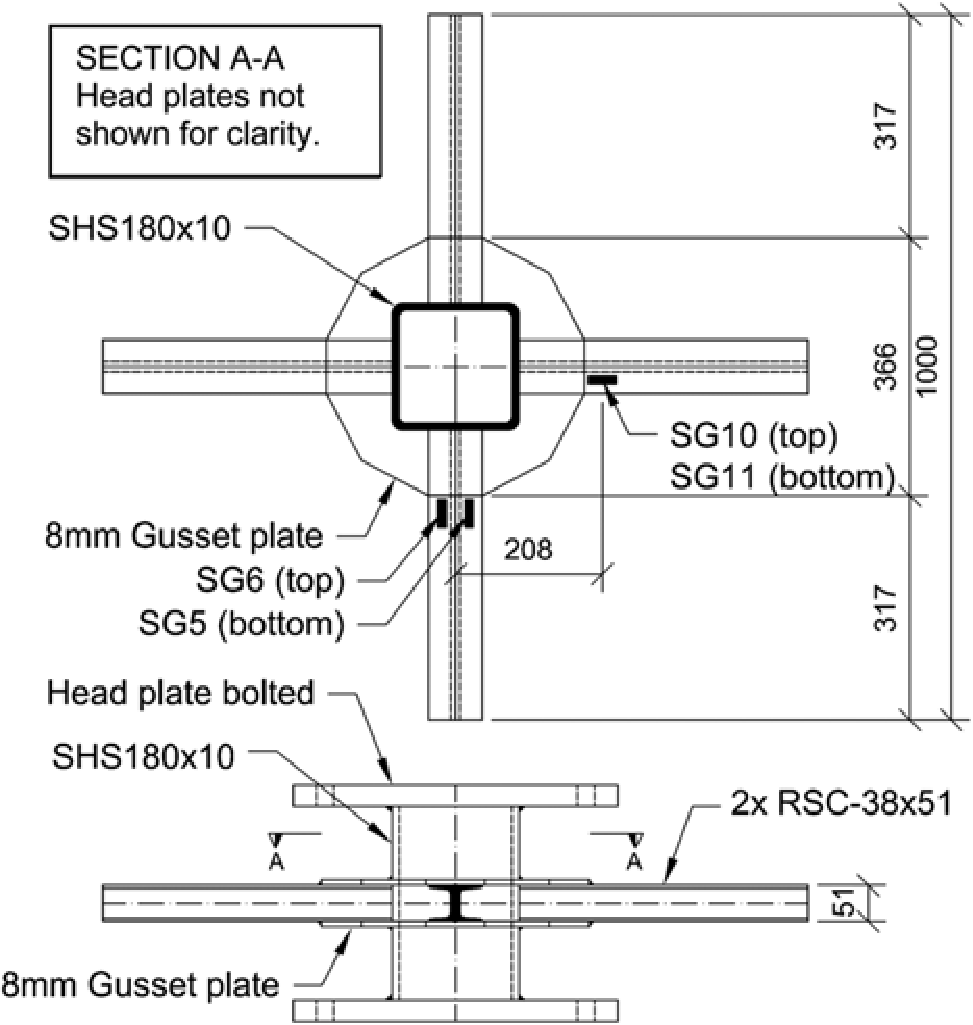
\includegraphics[width=\columnwidth]{Figures/e2011f4.pdf}
    \caption{Shearhead detail proposed in \cite{EDER20111164}.}
    \label{e2011f4}
    \end{figure}
\begin{figure}\centering
    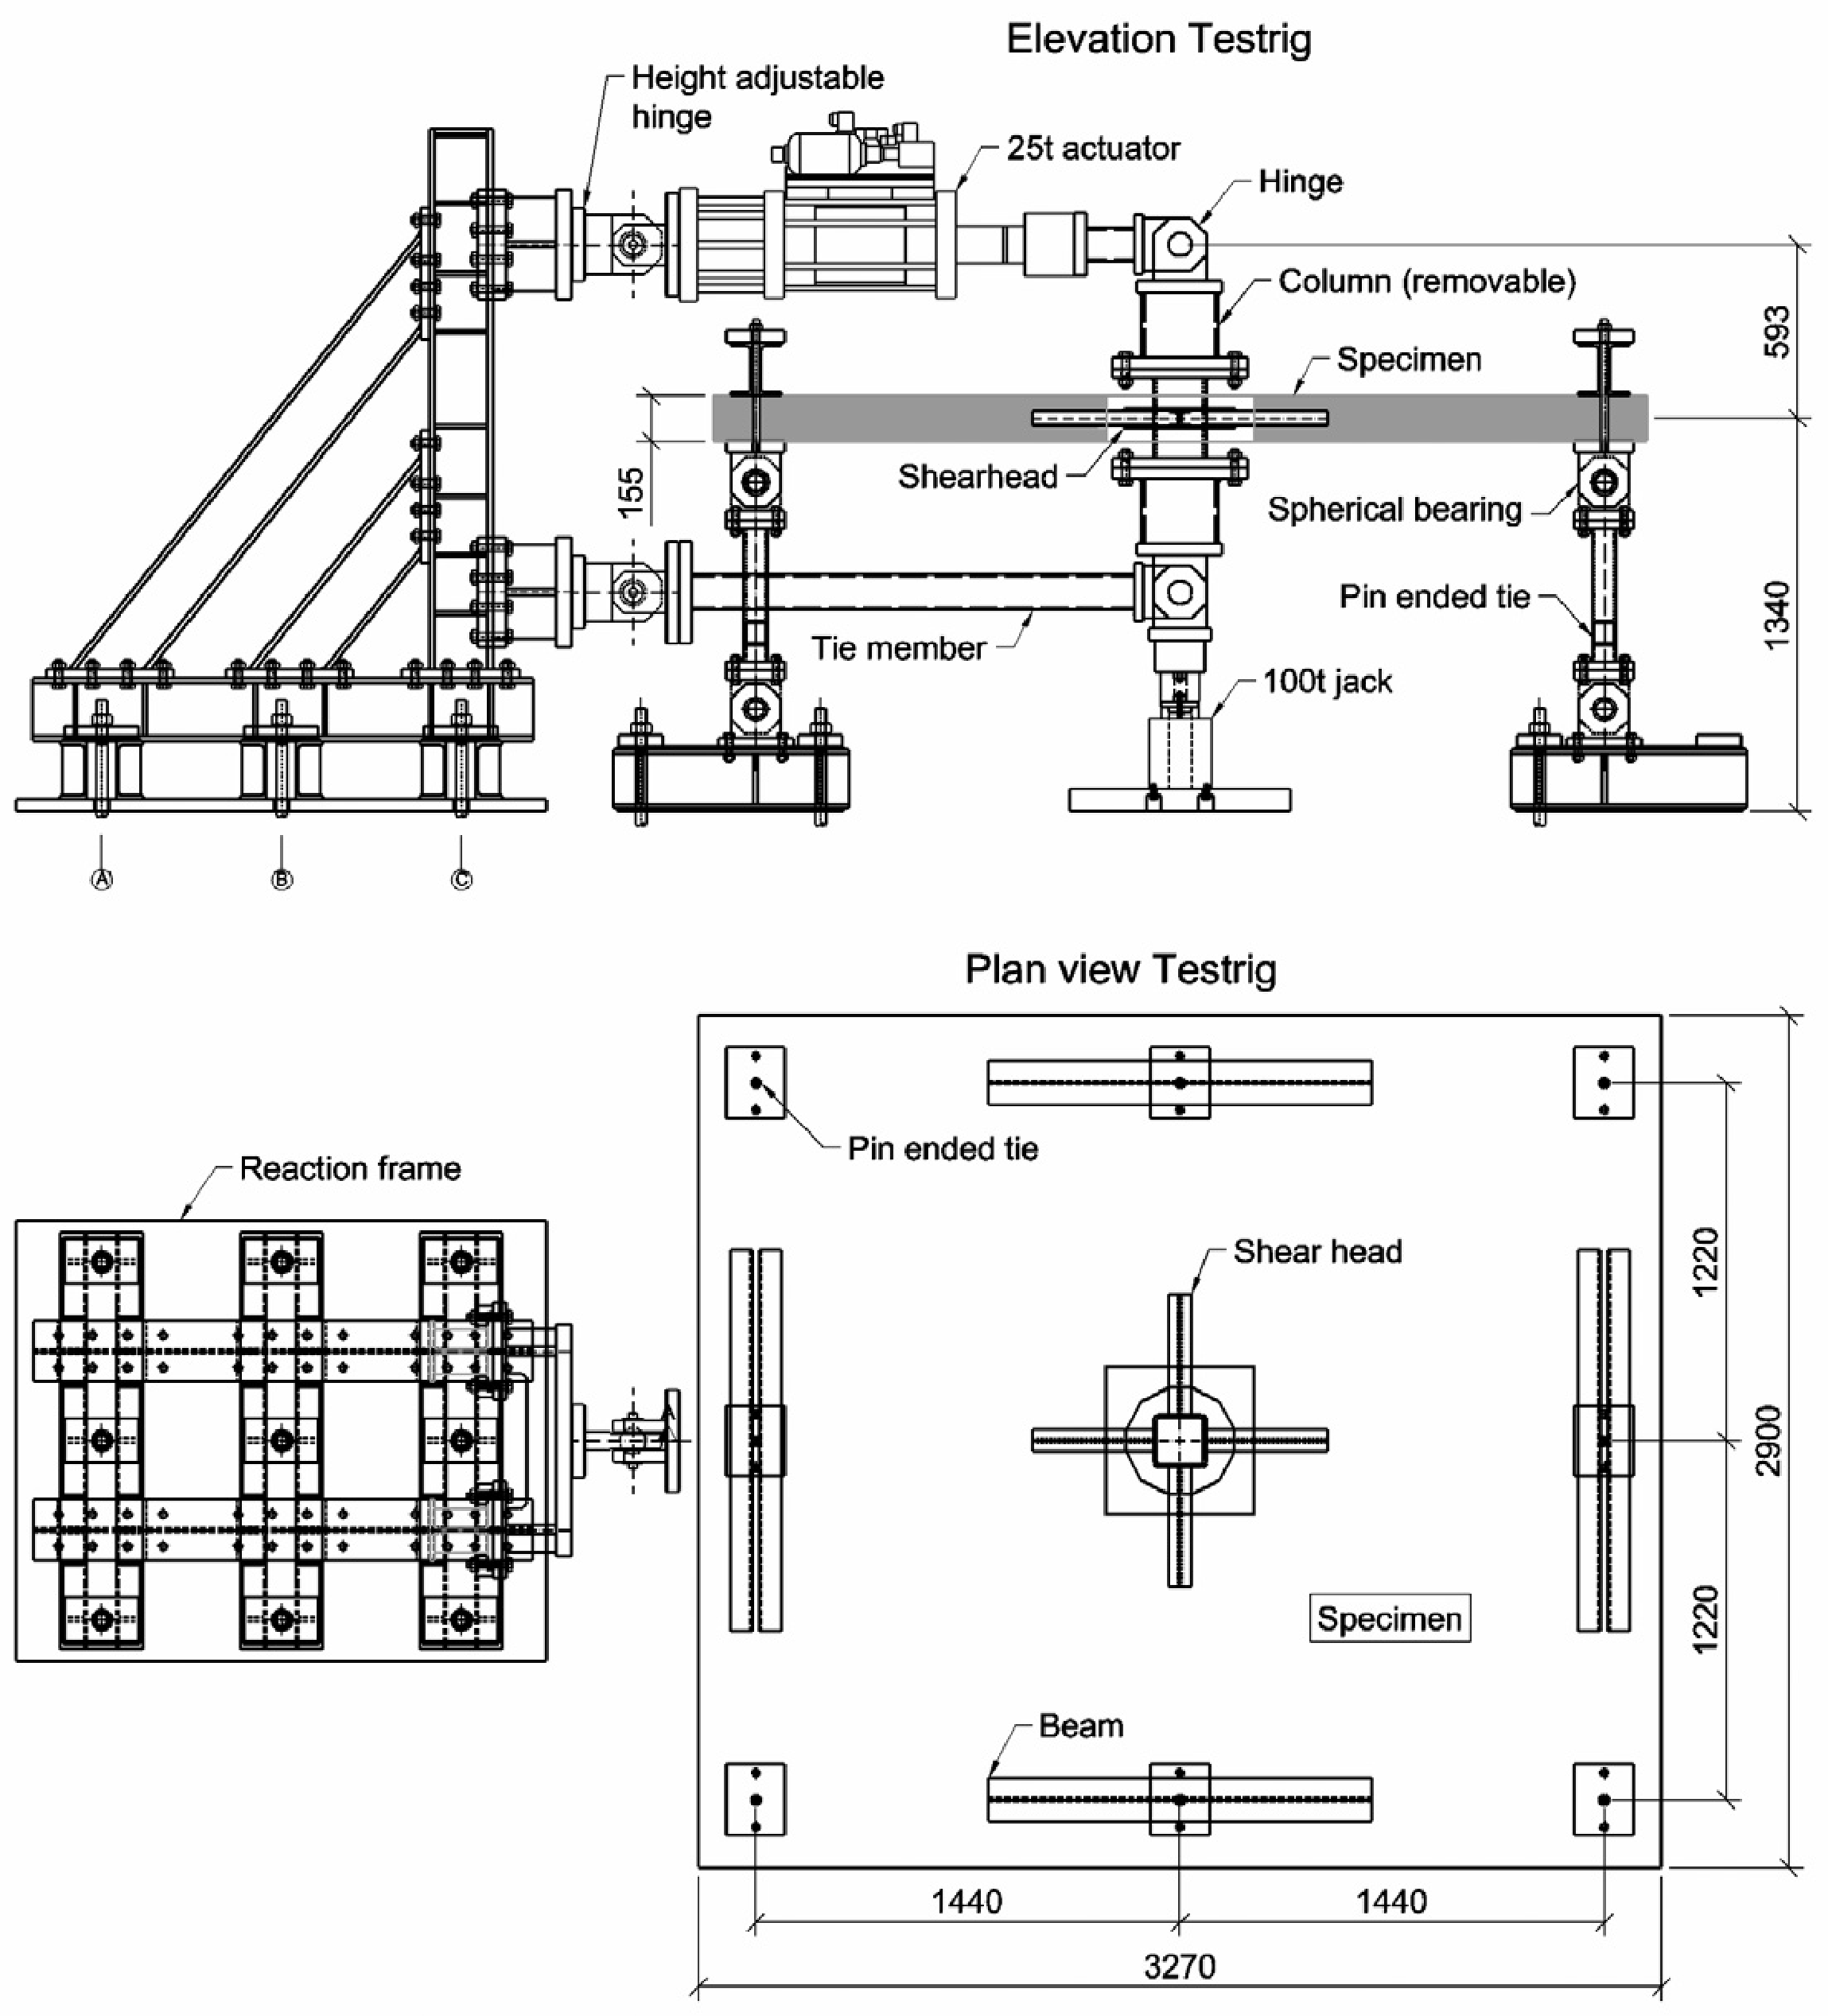
\includegraphics[width=\columnwidth]{Figures/e2012f1.pdf}
    \caption{Test rig used for large-scale tests\citep{EDER2012239}.}
    \label{e2012f1}
    \end{figure}

\subsubsection{Bent bars and stirrups}
\cite{bavzant1987size} improved understanding of member size effect on slab behavior with large scale specimens and proposal of a design formula. Following an experimental program \cite{shehata1989punching} presented a mechanical model to estimate punching shear resistance of axisymmetric slabs under concentric loads.  In order to analyse punching shear resistance of flat slabs with shear reinforcement \cite{gomes1999} proposed an analytical model based on \cite{kinnunen1960,shehata1989punching} validated on 12 full scale test specimens. \cite{birkle2008} focused on the influence of slab thickness while \cite{beutel2002} studied anchorage effect on shear reinforcement effectiveness over the shear punching critical section. Detailed investigations by \cite{guandalini2009punching,muttoni2008punching} resulted in a analytical model of punching shear strength as a function of slab rotation that formed the basis for \cite{mc2010} as well. \cite{ruiz2009} delved deeper into shear reinforcement contribution to punching shear strength based on slab rotation applying the critical shear crack theory. Several transverse reinforcement configurations were tested through 16 flat slab specimens with various depth by \cite{lips2012} to verify design effectiveness of methods presented in both the United States and Europe \cite{ACI-318M2014,en1992} in addition to the mechanical models presented in \cite{muttoni2008punching,ruiz2009}. Note that \cite{en1992} does not provide any design guidance for members with shearheads. 
\subsubsection{Headed studs}
Bent bars and stirrups make for rather tiresome to install shear reinforcement and this problem has caused the widespread use of shear studs (stud rails) during the recent decades. Several horizontal cyclic loading tests \cite{dilger1994,robertson2002,brown2003,broms2007ductility,tan2005interior,kang2008,hong2007lattice,matzke2015behavior,isufi2018} have investigated headed stud efficiency, placing it among the most effective and practical solutions for flat slab shear reinforcement(\ref{i2018f2}). \cite{ghali2005,hueste2007} attribute shear stud enhanced behavior to proper anchorage on both stud ends compared to other shear reinforcement. \cite{dam2016} presented the results of three full-scale slab-column connection test carried out to evaluate stud layout effectiveness in flat slabs with low flexural reinforcement(\ref{d2016f2}). \cite{dam2017punching} carried out seventeen large-scale tests of interior slab-column connections with different shear stud layouts and slab flexural reinforcements(\ref{d2017f3}).
\begin{figure}\centering
    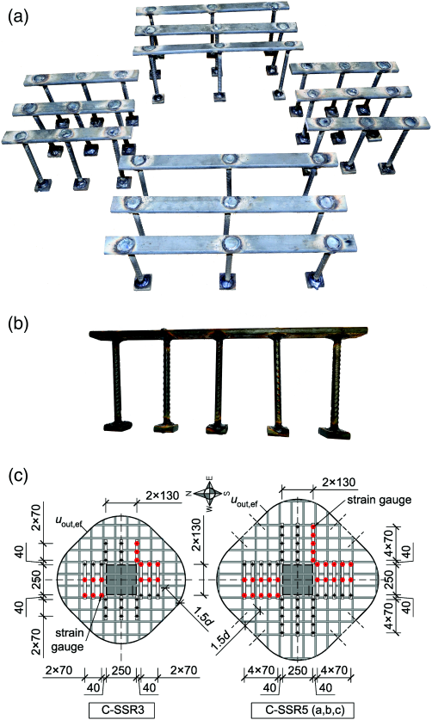
\includegraphics[width=\columnwidth]{Figures/i2018f2.png}
    \caption{Shear Studs\citep{isufi2018}: a) Complete set of studs for specimen C-SSR3; b) Stud rail along the longitudinal (N-S) direction for specimens with five rows of studs; c) Layout and instrumentation.}
    \label{i2018f2}
    \end{figure}

\begin{figure}\centering
    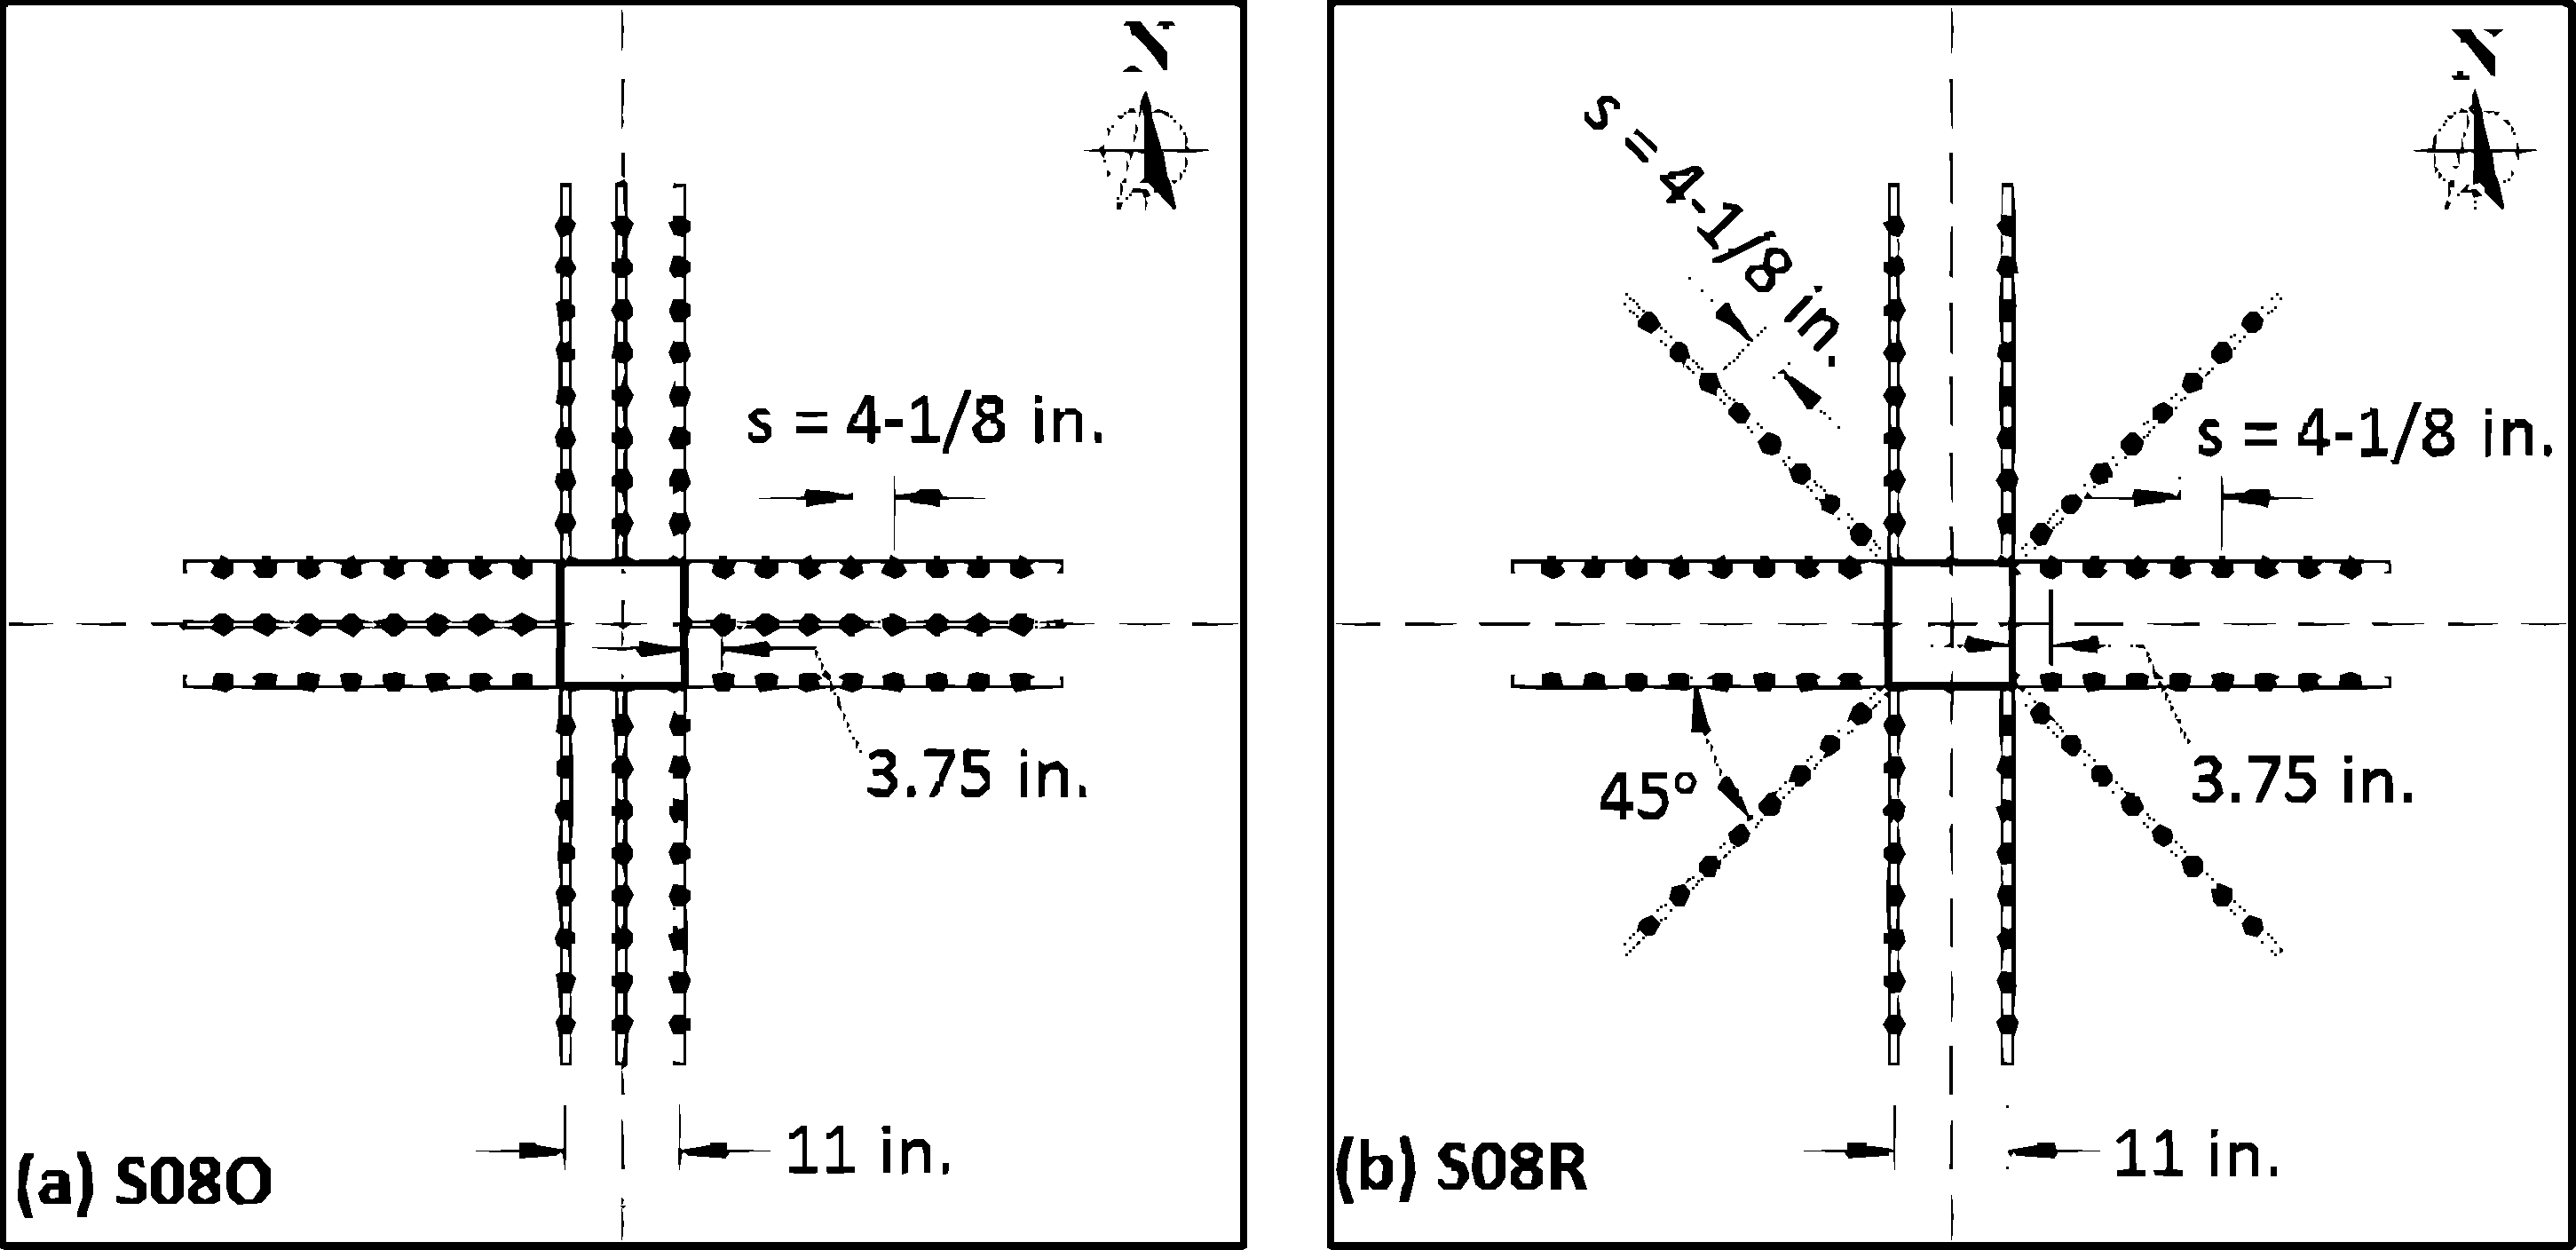
\includegraphics[width=\columnwidth]{Figures/d2016f2.pdf}
    \caption{Shear stud layouts in S08O and S08R specimens\citep{dam2016}.}
    \label{d2016f2}
    \end{figure}
    \begin{figure}\centering
        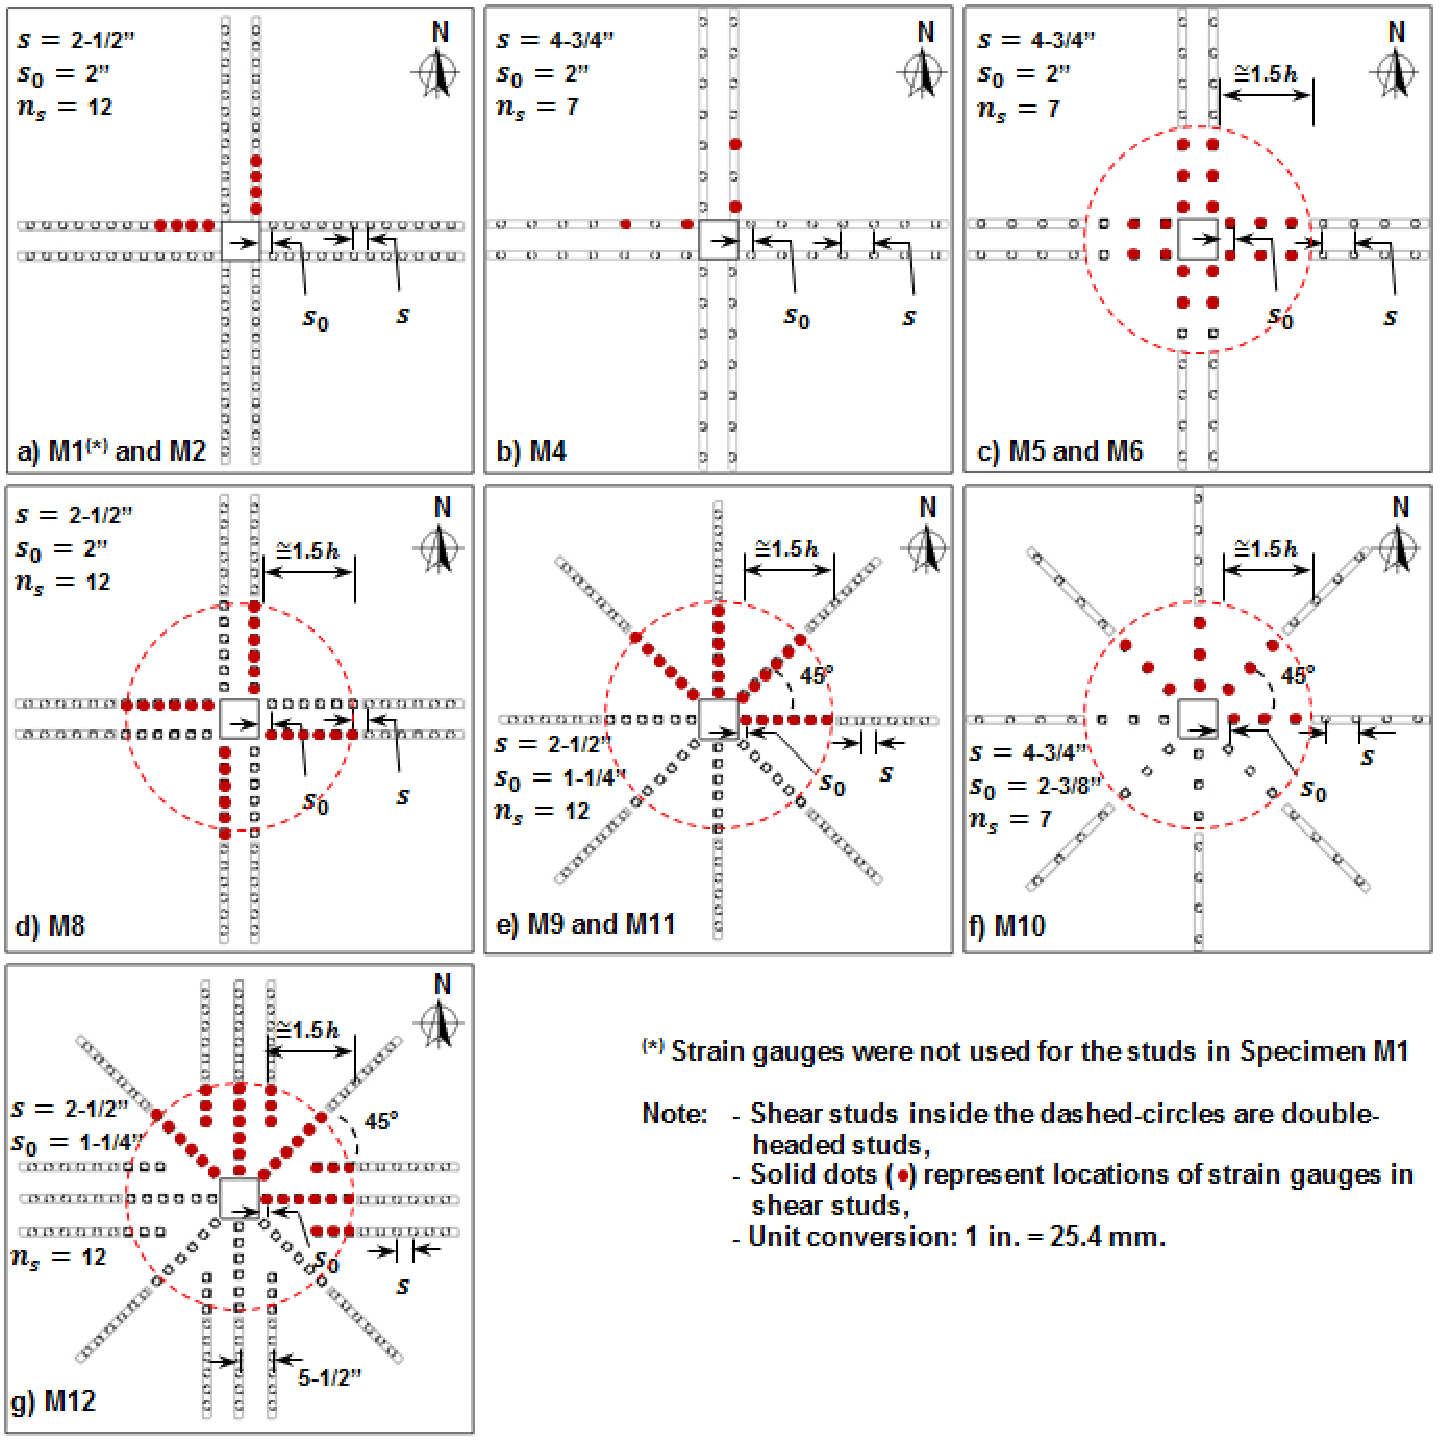
\includegraphics[width=\columnwidth]{Figures/d2017f3.pdf}
        \caption{Shear stud configurations and strain gauge locations for the M specimen series\citep{dam2017punching}.}
        \label{d2017f3}
        \end{figure}
        \cite{cho2009} compared a combination of steel plate and studs with stud rails in slab-column connections in which the former exhibited significantly higher ductility and punching shear capacity.
\cite{isufi2018} tested four reinforced concrete slabs with shear studs and a control specimen without any shear reinforcement under constant gravity loads and reversed horizontal cyclic displacements that differed in gravity load and stud perimeters. 
\subsection{Flexural reinforcement}
\cite{isufi2020} preformed combined horizontal reversed cyclic and gravity loading tests on two flat slab-column specimens with and without shear reinforcement and later continued with three more specimens in \cite{isufi2021} to better study flexural reinforcement(\ref{i2021f1}) influence on flat slab-column connection seismic performance which was aligned with previous results\citep{muttoni2008punching,guandalini2009punching,ghali2019,torabian2019} indicating that flexure rather than punching shear governs slab load carrying capacity with flexural reinforcement decrease. Low reinforcement ratios lead to flexural reinforcement yield onset and a more ductile behavior from the slab until shear crack widening at relatively large displacements ends in punching\citep{muttoni2008punching,torabian2020,torabian2019}. The importance of flexural reinforcement was noted earlier tests as well\citep{hawkins1974w,symonds1976}. \cite{morrison1983lateral} tested five relatively thin slab-column connection specimens, three of which had different flexural reinforcement ratios and their response was dominated by flexure since these specimens were tested without gravity load allowing high ultimate drift capacity. \cite{morrison1983lateral} Notes theoretical yield onset for the lowest flexural reinforcement specimen. \cite{emam1997seismic,marzouk2001cyclic} investigated flexural reinforcement influence on slab-column connection seismic behavior. Detailing of top and bottom reinforcement of slab-column connection under lateral cyclic loading was studied by \cite{Robertson2006} with six specimens that showed horizontal load bearing capacity improvement by flexural reinforcement increase while deformation capacity could be hindered by premature punching shear.  Five specimens with different flexural reinforcement were tested by \cite{tian2008behavior} one with reversed horizontal cyclic loading to failure and two with gravity loading to failure after undergoing a cyclic loading protocol, that exhibited punching shear capacity increase under gravity load and lateral stiffness increase under horizontal load with flexural reinforcement increase. A total of 13 internal slab-column connection specimen test were conducted by \cite{drakatos2016} in which monotonic and reversed cyclic loading, gravity load and flexural reinforcement varied. Slab-column connection lateral stiffness improved with flexural reinforcement increase while its influence on unbalanced moment and deformation capacities remained heavily dependent on applied gravity load levels for monotonic lateral loading, also cyclic loading affected slabs with higher flexural reinforcement ratios less than those with lower ratios. 
\begin{figure}\centering
    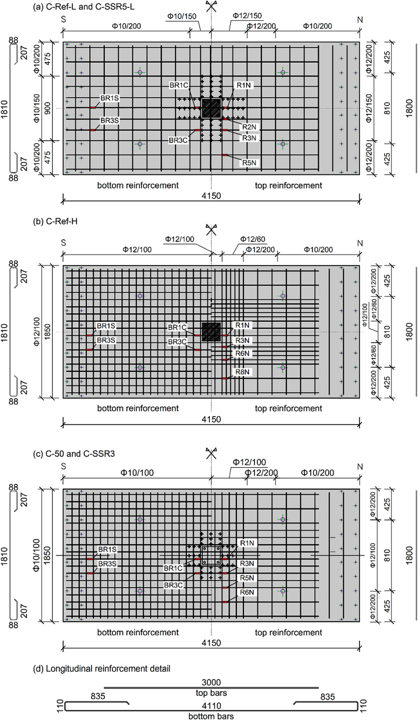
\includegraphics[width=\columnwidth]{Figures/i2021f1.png}
    \caption{Flexural reinforcement details\citep{isufi2021}.}
    \label{i2021f1}
    \end{figure}